\documentclass{beamer}
\usepackage[english]{babel}
\usepackage{geometry}
\usepackage[utf8]{inputenc}
\usepackage{colortbl}
\usepackage{natbib}
\usepackage{listings}
\usepackage{adjustbox}
\usepackage{verbatim}
\usepackage{amsmath}
\usepackage{multirow}
\usepackage{makecell}
\usepackage{tabularx}
\usepackage{tikz}
\usepackage[linewidth=1pt]{mdframed}
\usepackage[utf8]{inputenc}
\usepackage[absolute,overlay]{textpos}
\usepackage{listings}
\usepackage{color}
\usepackage{minted}
\usepackage{multimedia}
\usepackage{eso-pic}
\usepackage{pgfpages}
%\setbeameroption{show notes on second screen=bottom} %

% minted styles
\setminted[csharp]{escapeinside={*@}{@*}}
\newmintinline[csharpinline]{minted-lexers/csharp.py:MDCSharpLexer -x}{breaklines}
\newminted[mintedcsharp]{minted-lexers/csharp.py:MDCSharpLexer -x}
{
frame=single,
framesep=2mm,
baselinestretch=1.0,
bgcolor=backcolour,
fontsize=\tiny,
numbersep=0.1mm,
linenos,
framerule= 0.1pt,
breaklines,
autogobble
}

% Colors
\definecolor{dkgreen}{rgb}{0,0.6,0}
\definecolor{gray}{rgb}{0.5,0.5,0.5}
\definecolor{mauve}{rgb}{0.58,0,0.82}

\definecolor{codegreen}{rgb}{0,0.6,0}
\definecolor{codegray}{rgb}{0.5,0.5,0.5}
\definecolor{codepurple}{rgb}{0.58,0,0.82}
\definecolor{codeblue}{rgb}{0,0,0.95}
\definecolor{backcolour}{rgb}{0.95,0.95,0.95}

\definecolor{graph_isready}{HTML}{00ffff}
\definecolor{graph_active}{HTML}{cdad00}
\definecolor{graph_inactive}{HTML}{ee6a50}
\definecolor{graph_done}{HTML}{76ee00}
\definecolor{graph_waiting}{HTML}{ffffff}

% Define color boxes
\newcommand\textcolorbox[2][]{\tikz[overlay]\node[inner sep=2pt, anchor=text, rectangle,draw=black,thick , rounded corners=2mm,#1] {#2};\phantom{#2}}
\newcommand\statecolorbox[1]{\textcolorbox[fill=#1]{\phantom{\boxfillertext}}}
\newcommand\statecolorboxtext[2]{\textcolorbox[fill=#1]{\phantom{Xj}#2\phantom{Xj}}}
\newcommand{\boxfillertext}{XXX}

% Define images over each other
\newlength{\displayThumbnail}
\setlength{\displayThumbnail}{2cm}
%\def\Put(#1,#2)#3{\leavevmode\makebox(0,0){\put(#1,#2){#3}}}
%\newcommand\AtPagemyUpperLeft[1]{\AtPageLowerLeft{%
%\put(\LenToUnit{0.9\paperwidth},\LenToUnit{0.9\paperheight}){#1}}}

\usetheme{Madrid}
% \usefonttheme{structuresmallcapsserif}
% \usecolortheme{Copenhagen}

\usenavigationsymbolstemplate{} % no navigation buttons
% \usecolortheme{beaver}

% \setbeamercolor{block title}{bg=red!30,fg=black}


\title{TCP/IP in hardware using SME}
\author{Mark Jan Jacobi \& Jan Meznik}
\institute{KU}
\date{\today}


\begin{document}
\frame{\titlepage}
\note{\textbf{Mark} siger introduktion og 2-3 saetninger "abstrakt" }


\begin{frame}
    \frametitle{Table of Contents}
    \tableofcontents[hideallsubsections]
\end{frame}
\AtBeginSection[]
{
  \begin{frame}
    \frametitle{Table of Contents}
    \tableofcontents[subsectionstyle=shaded/show/hide,sectionstyle=show/shaded]
  \end{frame}
}

\section{Introduction}
\begin{frame}
  \frametitle{Background and Motivation}

FPGAs are making their way into data centers to boost the computing power
	and the overall power efficiency.


\begin{columns}
\begin{column}{0.8\textwidth}
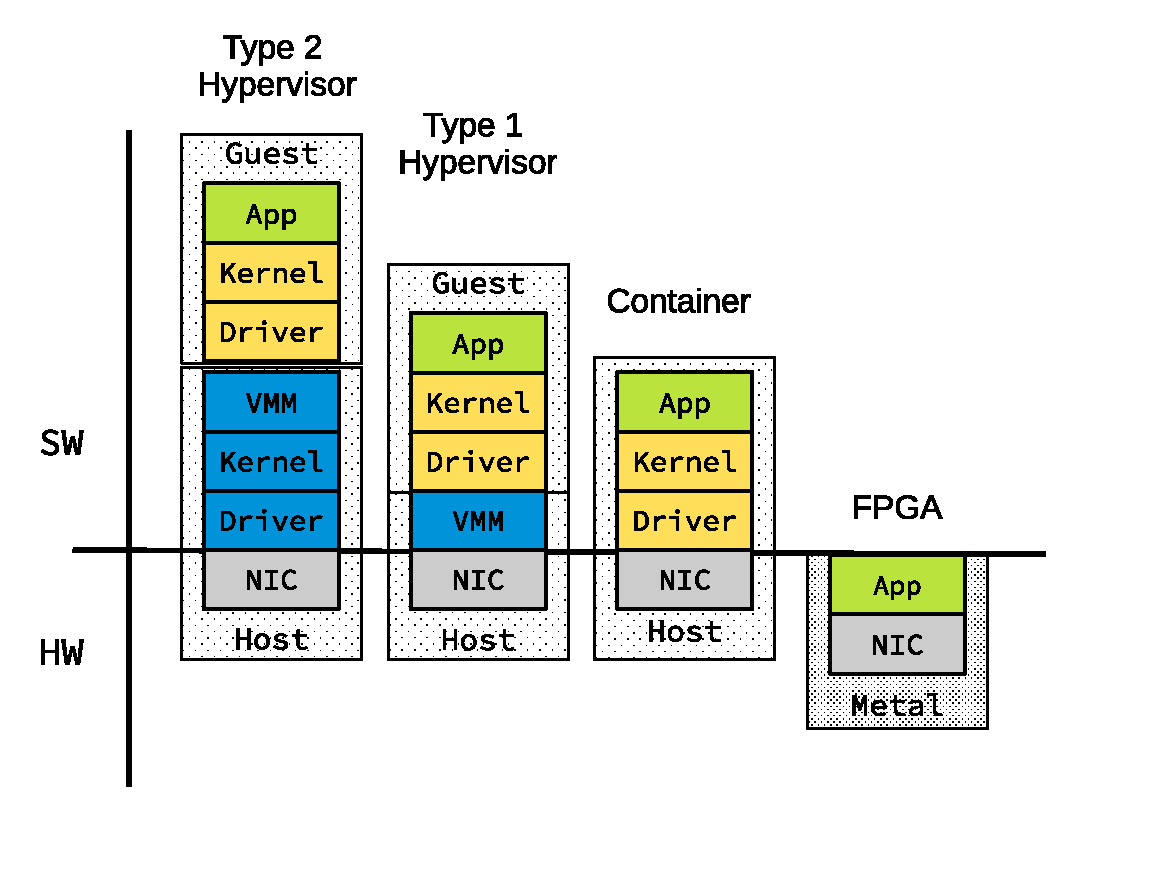
\includegraphics[scale=0.5]{./background/server_configuration.eps}
\end{column}

\begin{column}{0.2\textwidth}
\includegraphics[scale=0.2]{./background/intel_fpga_nic.jpg}
\end{column}
\end{columns}

\end{frame}




\note{Applikationer og Big-Data udregninger flytter til Cloud, drevet af store
data centre.\\

Disse data-centre kraever rigtigt meget plads, store maengder af stroem og er i stigende grad svaere
at vedligeholde og udvide.\\

De fleste data-centre er derfor begyndt at aflaste beregningerne til FPGAer,
som fjerner meget af overhead til beregningerne\\

kan bruges til at få en computer til at køre hurtigere hvis de mest brugte
instruktioner, skrives direkte ned i hardwaren\\

PROBLEMET er at der kun kan vaere en begreanset antal af FPGAer i konventionele
servere

}



% Talking points:


% > In the current era of big data, computationally heavy applications are
% moving to the cloud. ... Consuming wast amount of energy and are increasingly
% complex to maintain and improve

% > To combat this, DC servers offload the computation onto FPGAs

% <SHOW GRAPH HERE>

% > However, this is not scalable in the conventional DC architecture, as the
% FPGAs are directly connected to CPUs using a PCI bus.

% <SHOW CONVENTIONAL DC>

% > Disaggregated DC architecture proposes FPGA be turned into a
% self-contained standalone appliance capable of managing itself. Then, it is
% connected to the rest of the Data-Center by a local network. This enables the
% DC to pack even more computing capacity into the same physical volume at the
% same, or even lower, energy consumption.

% <SHOW DISAGGREGATED DC>

% > This can increase the density of the servers by sharing resources
% such as power supplies, cooling, fans, networking uplinks, and other management
% infrastructures.

% > In this thesis, we want to make a self-contained TCP/IP stack on an FPGA
% using SME.



\begin{frame}

A conventional data center architecture
\begin{figure}
	\centering
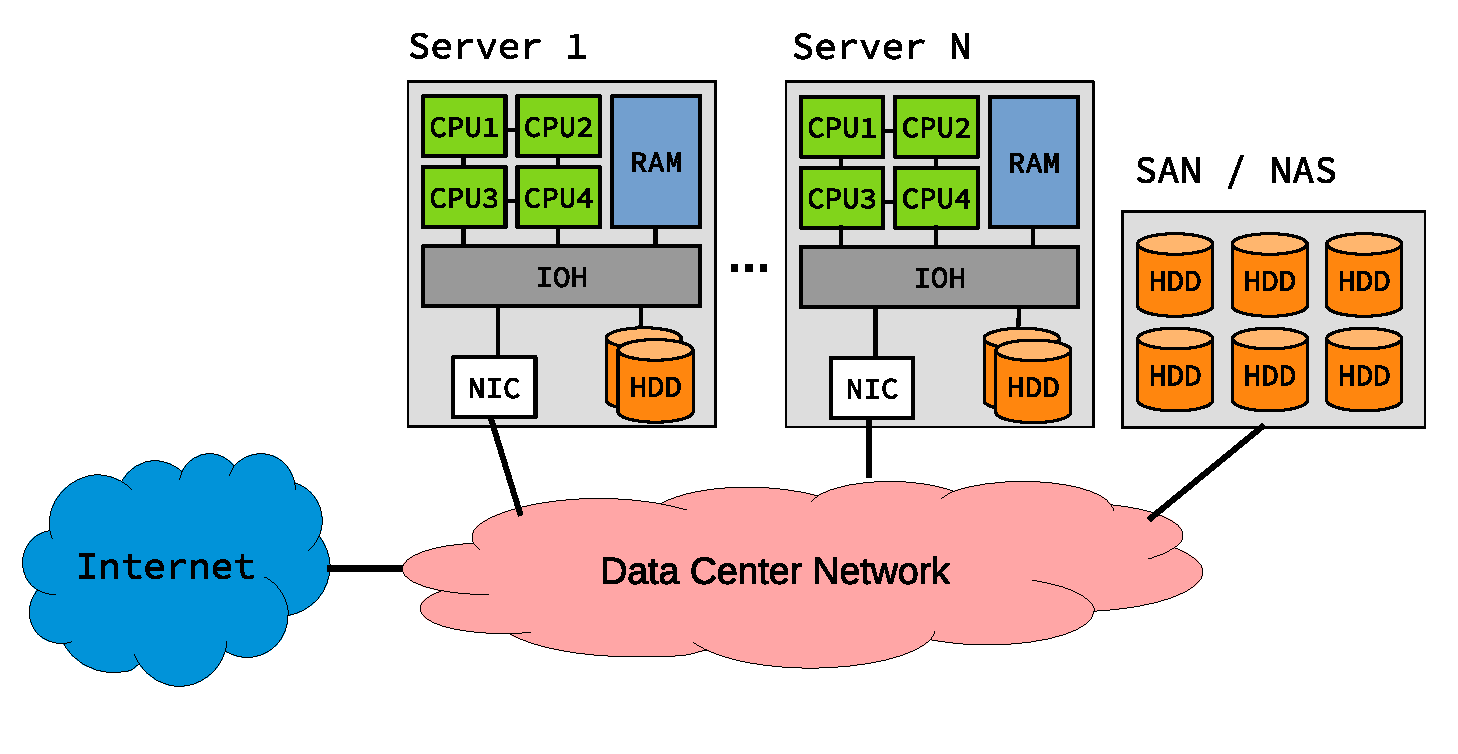
\includegraphics[scale=0.5]{./background/dc_architectures_conventional.eps}

\end{figure}

\end{frame}


\begin{frame}
	Proposed disaggregated data center architecture (\cite{7830659})
\begin{figure}
	\centering
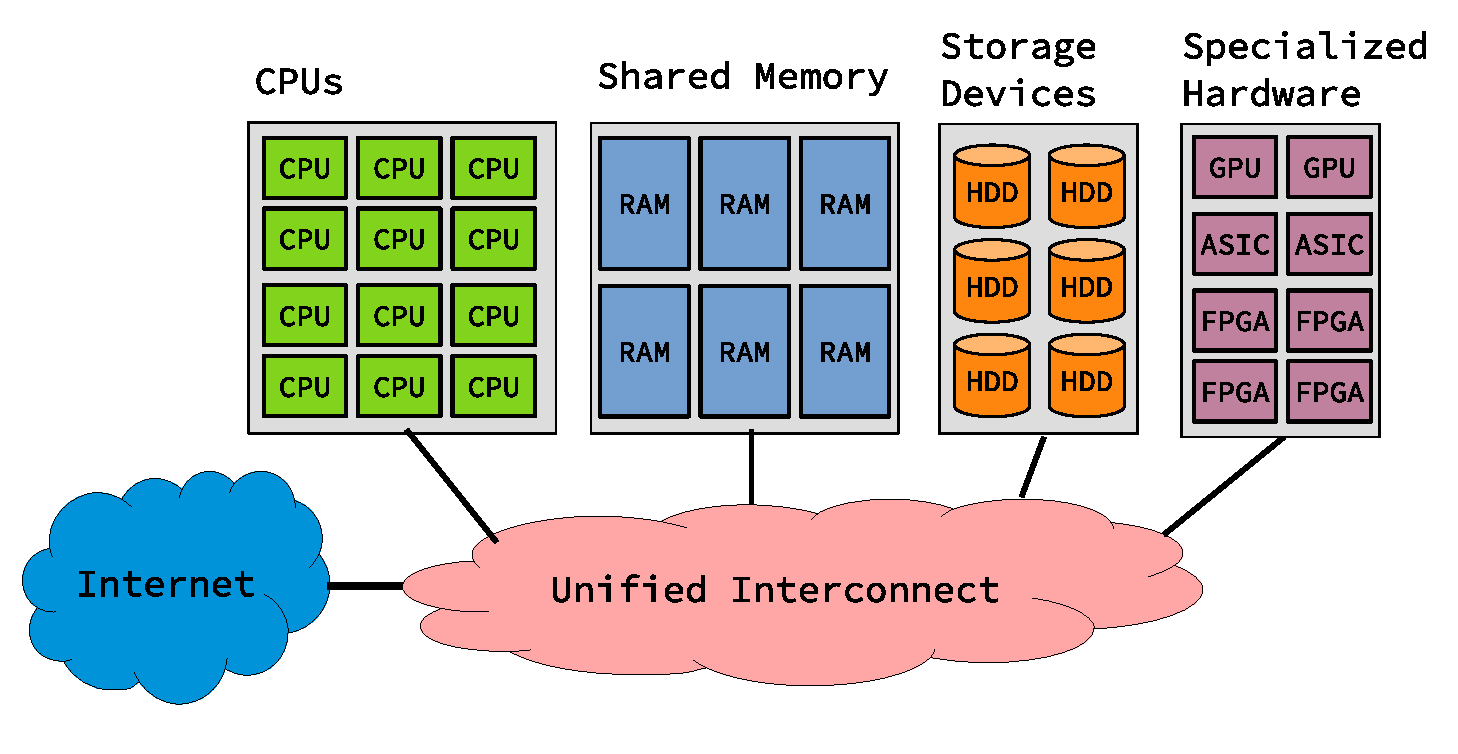
\includegraphics[scale=0.5]{./background/dc_architectures_disaggregated.eps}
\end{figure}
\end{frame}

\note{Hvis man splitter resourcerne op, kan man takket været FPGA få bedre
ydeevne på det samme areal, samt nemmere håndtering af servere og deres komponenter. }

\begin{frame}
FPGA usage
\begin{figure}
	\centering
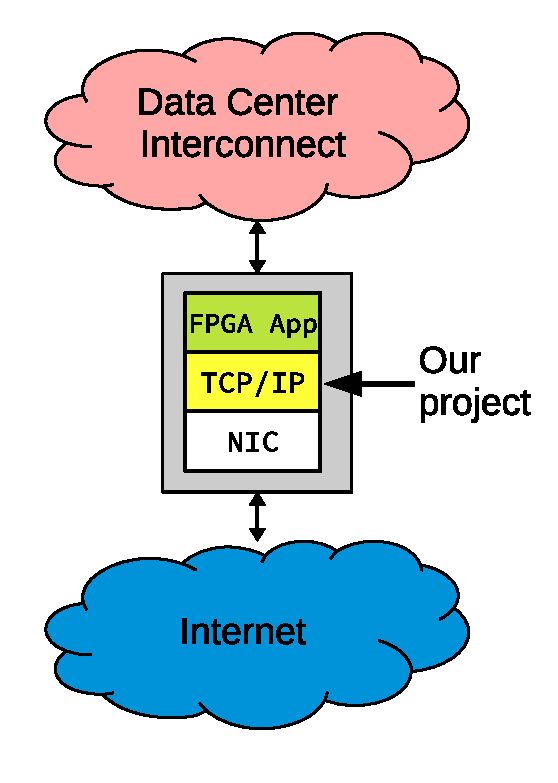
\includegraphics[scale=0.5]{./background/fpga_usage.eps}
\end{figure}

\end{frame}

\begin{frame}
The Internet

\begin{figure}
	\centering
\includegraphics[scale=0.18]{./background/internet_map.jpg}
\label{fig: Internet map}
\caption{Map of the 30\% of accessible the endpoints on the Internet}
\end{figure}

\end{frame}


\begin{frame}
The Internet Protocol Suite -- A scenario
\begin{figure}
	\centering
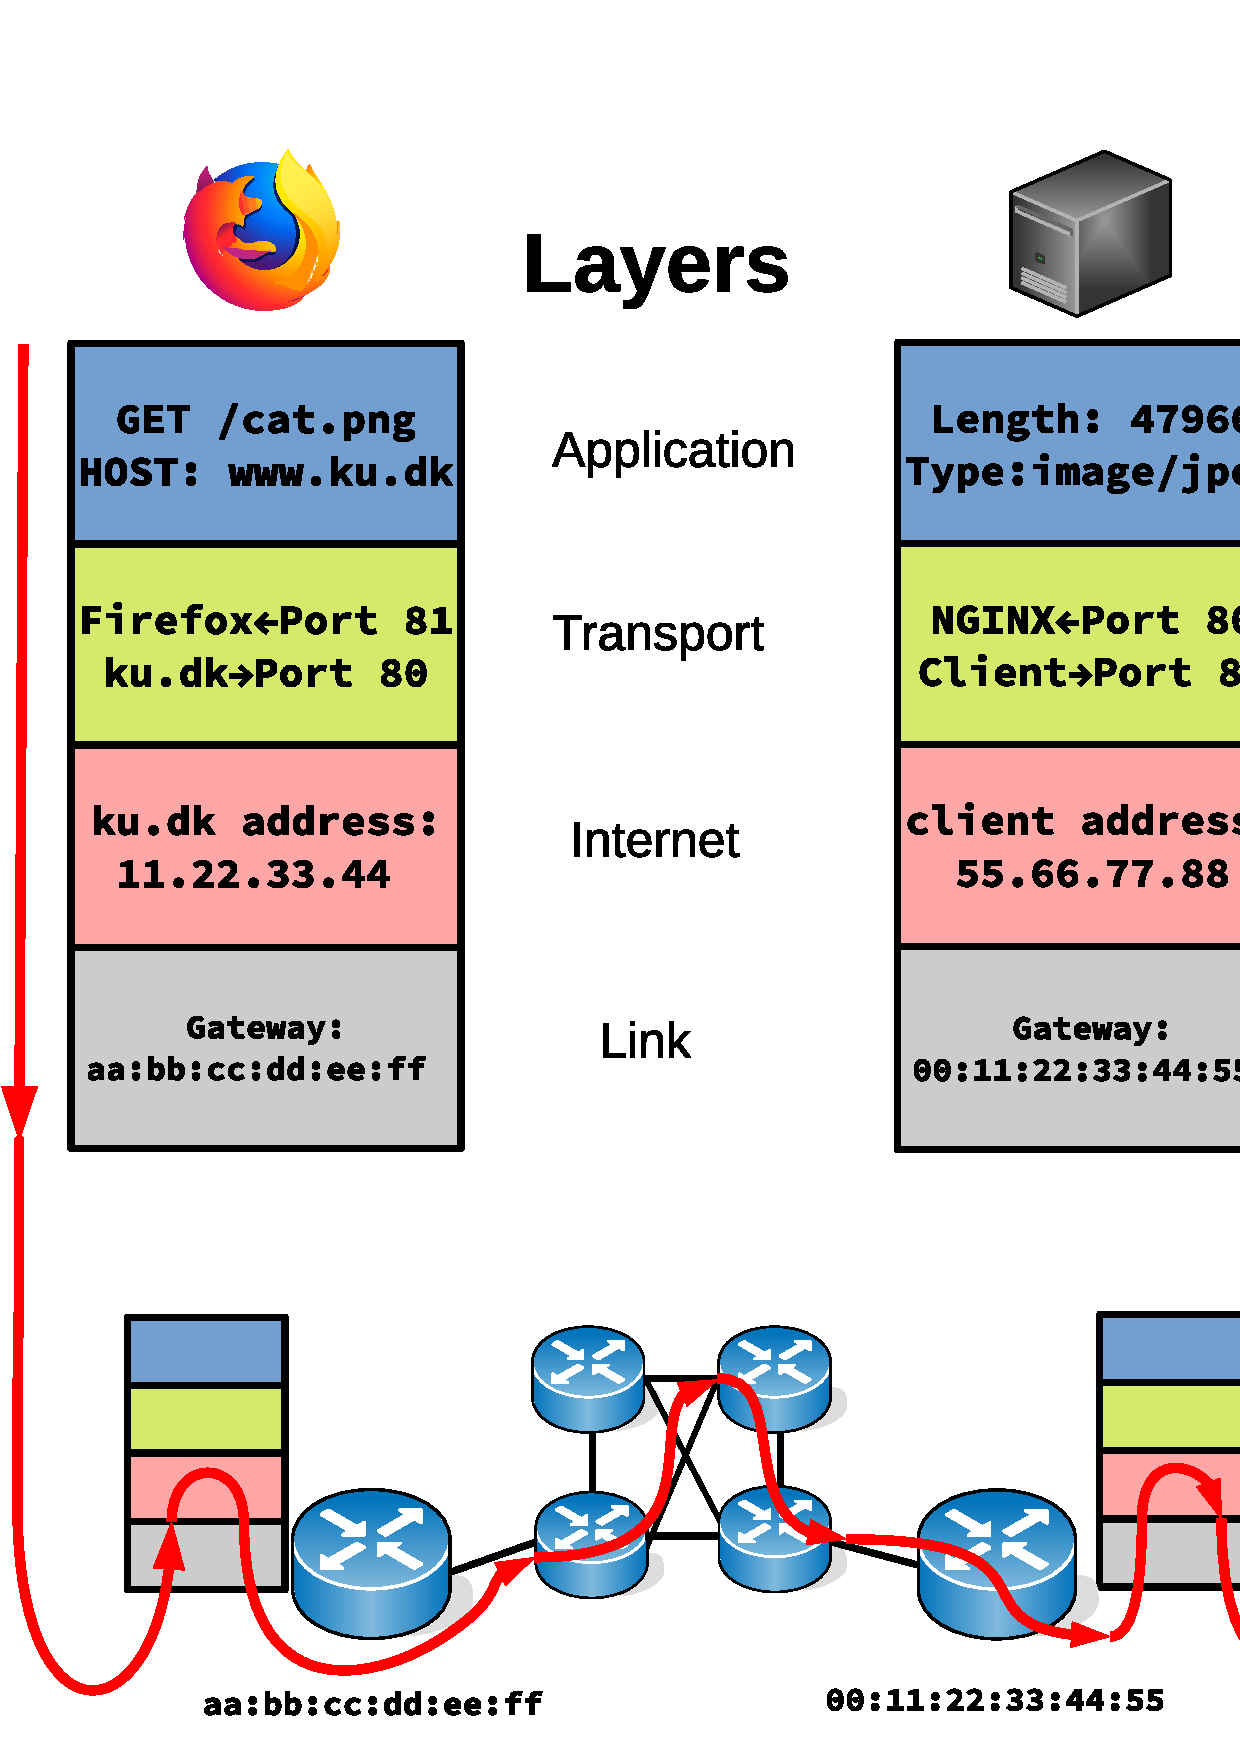
\includegraphics[scale=0.28]{./background/internet_scenario.pdf}
\end{figure}



\end{frame}


\begin{frame}
Design with the 4 layers in mind
\begin{figure}
	\centering
%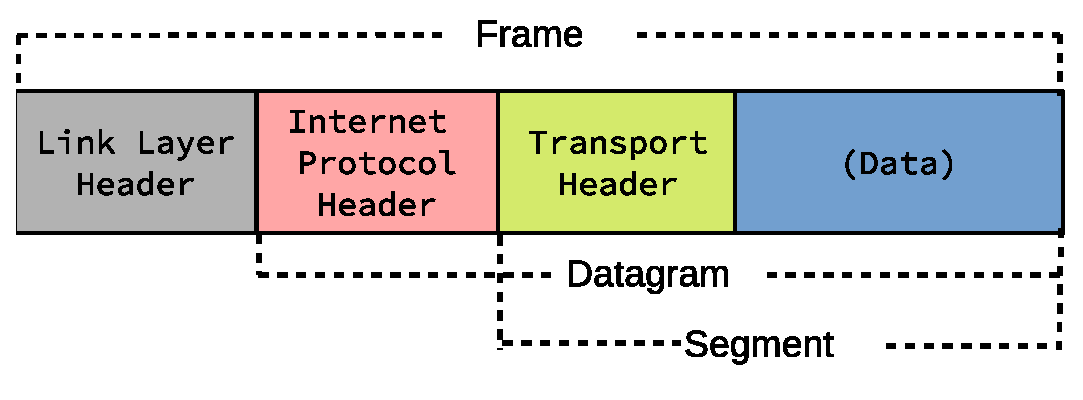
\includegraphics[scale=0.5]{./background/frame.eps}
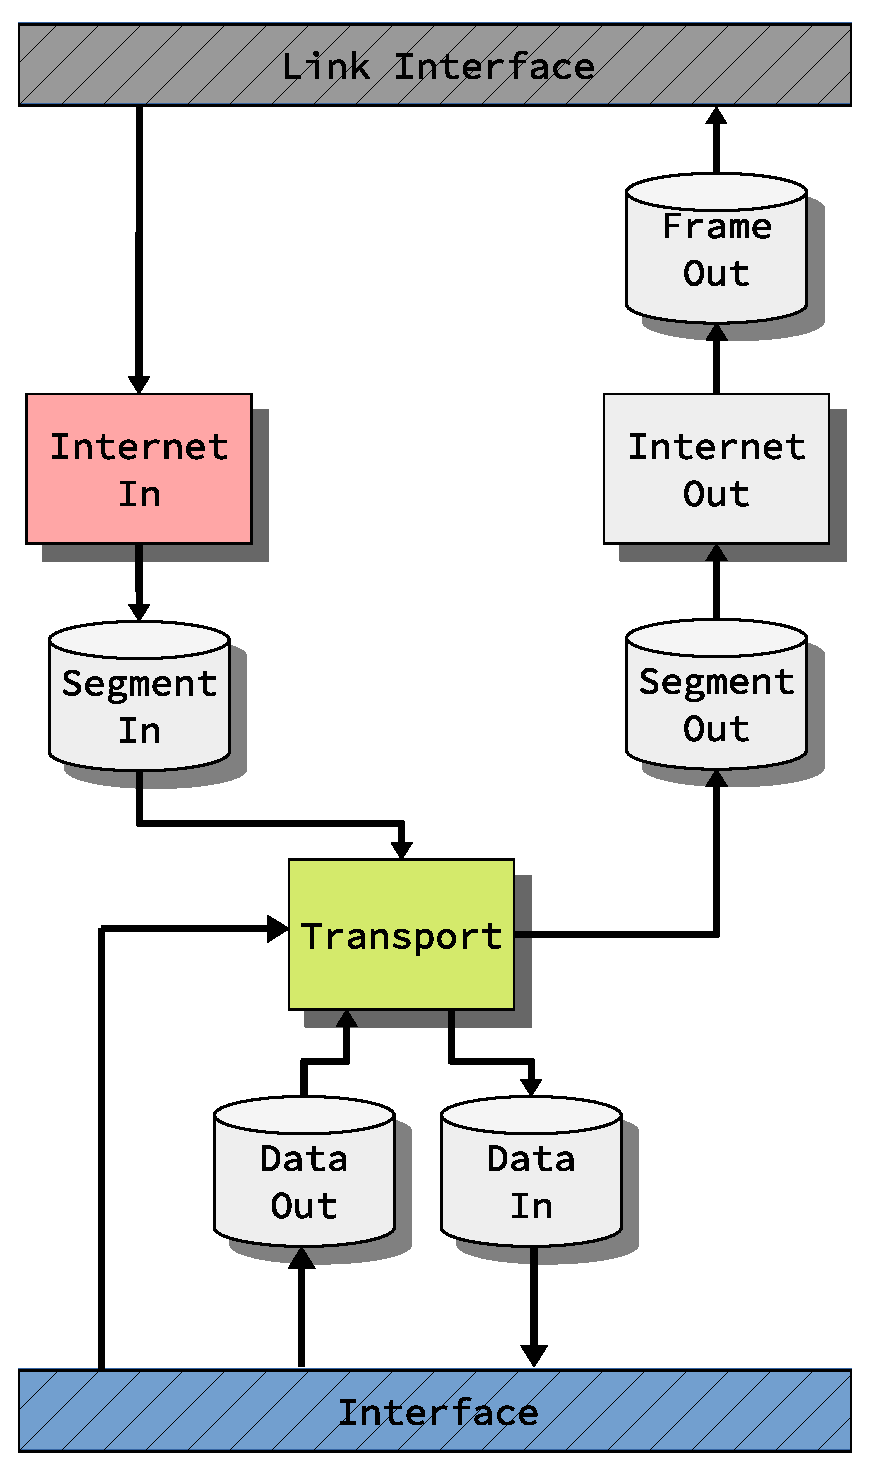
\includegraphics[scale=0.3]{./background/design_2.eps}
\end{figure}
\end{frame}



% - Network Stack Specialization for Performance\\
% - Disaggregated FPGAs\\
% - A Cloud-Scale Acceleration Architecture

% Talking points:
% 1. In the current era of big data, computationally heavy applications are
% moving to the cloud.

% 2. DC infrastructures are being redesigned to pack ever more compute capacity
% into the same volume and power envelops

% 3. This is done by increasing the density of the servers by sharing resources,
% such as power supplies, cooling, fans, networking uplinks, and other management
% infrastructures.

% 4. Problem -- currently, FPGAs are connected directly to CPUs using some PCI
% bus, making the separation hard. [0] proposes FPGA must be turned into a
% self-contained standalone appliance capable of managing itself. Then, it is
% connected to the rest of the Data-Center by a local network.

% 5. In this thesis, we want to make a self-contained TCP/IP stack on an FPGA
% using SME.


% [0]: [Disaggregated FPGAs]



\chapter{Design}
% introduction about the network stack?

\section{Overview}
The networking stack introduced in this thesis is implemented in the C\# 
programming language with SME. The aim of its design is to capacitate performance,
flexibility, and ease of use. In this chapter, the design principles are 
described, the architecture of the solution is outlined, and the components are
outlined.


\subsection{Design principles}
As briefly mentioned in the introduction, the proposed network stack is to 
provide an alternative to the existing proprietary network offloading engines.
While the main goal of this thesis is to research and study the suitability of 
SME for implementing a TCP/IP stack on an FPGA, there are many other aspects of the 
system to be studied.\\
The extensibility of the network stack are to be tested by studying the effects 
of introducing new protocols to the stack. While the network stack should be 
able to be refined with new and custom protocols, it is to be studied which 
implications it has for the system. Mainly, it is to be seen how the addition 
of new protocols affect the performance, scalability, and viability of the 
system.\\
In the same vein, the design should be as FPGA-agnostic as possible. While this is 
mainly guaranteed by the SME framework used to develop the system, the underlying
systems, operations, and features should be easily portable across FPGA manufacturers.\\
Lastly, the design of the networking stack should be interoperable with other 
systems on the FPGA, or even FPGAs. It is to be seen how easy it us to modify
and extend the versatility of the system without any major modifications or 
even extensible knowledge of the system. As an example, the networking stack 
can be expanded with a firewall, developed alongside this project. 

\subsection{Initial requirements}
Following our design principles, initial requirements and goals for the 
networking stack are set so that these can be tested and improved upon. 
\begin{itemize}
\item \textbf{Essential protocols only}\\
Considering that the SME project is still fairly early in its development, and considering 
the sheer number of protocols in the internet protocol suite, the networking 
stack in this thesis is to support only the absolutely essential protocols 
required to provide the users with a meaningful interface to the internet.
These protocols should be picked such that the system can provide the end-user
with a network data-stream, which can transport information to and from a remote
computer.\\
The initial protocols chosen may be implemented and supported partially, but 
they must not deviate from the standard specifications. 

\item \textbf{Support an interface for the end-user}\\
The system must be controlled by an end-user on the FPGA. Such an interface is 
very unique in its own way, compared to standard software interfaces, like the 
ones defined in the POSIX collection of specifications. By supporting such an
external interface gains insight in the way such a networking stack will be used,
and which measures must be taken in order to provide the best possible integration
and performance considerations.

\item \textbf{Independent of underlying physical hardware}\\
By using SME, the underlying hardware description language code can be abstracted
away from the actual implementation. This will later provide developers to easily
modify and tweak the networking stack without having to consider the target 
hardware.\\
Likewise, the networking stack may not rely on using a certain physical layer hardware,
and must be designed to be independent of the underlying hardware used for the 
physical connections. This will ensure that the target hardware can easily 
swap between physical connectors, such as going from ethernet cables to wireless,
or even another FPGA.
\end{itemize}

\section{The architecture}
\subsection{Initi1al design}

\begin{figure}
    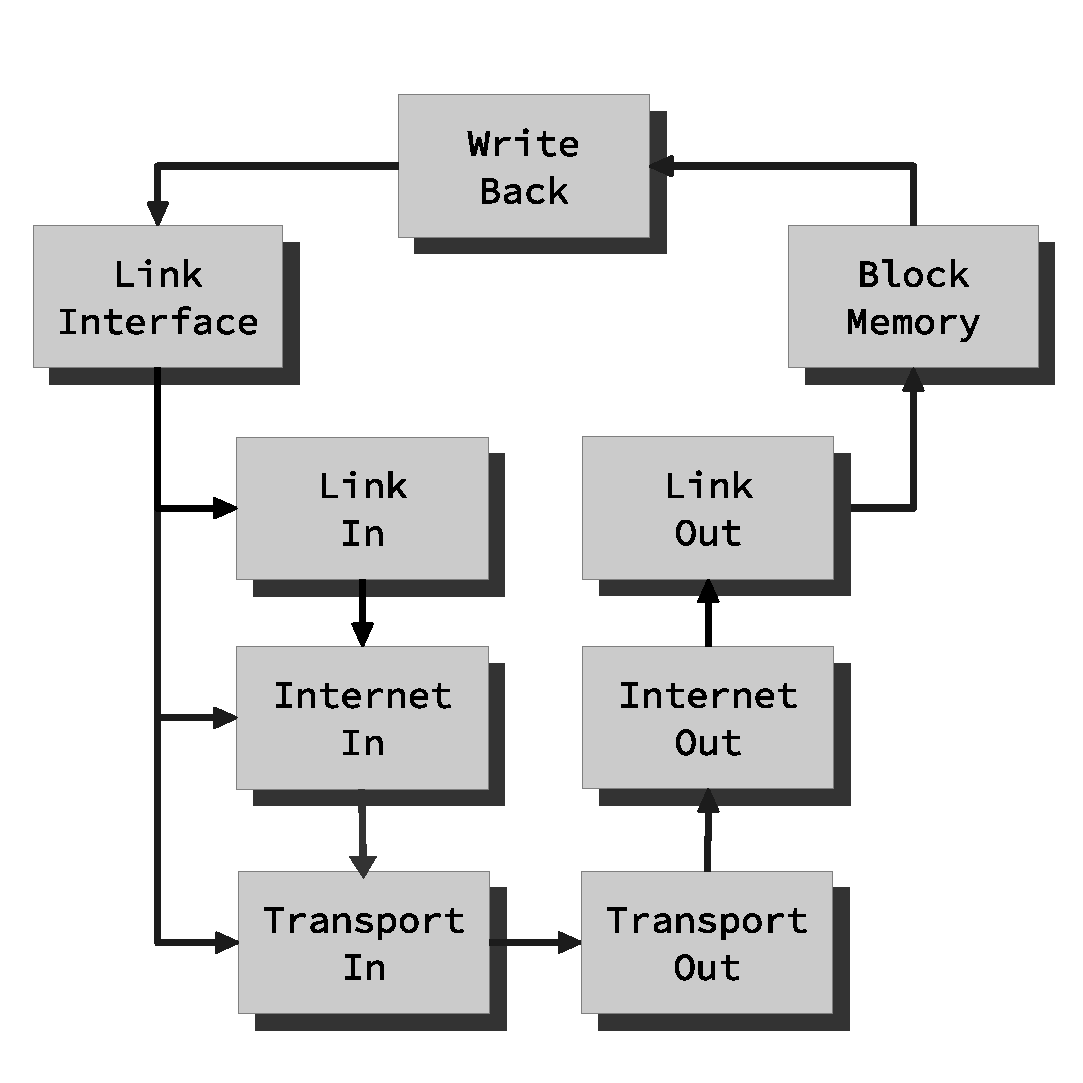
\includegraphics[scale=0.45]{design/design_0.eps}
    \caption{The initial design}
    \label{fig:initial_design}
\end{figure}

The initial architecture focused heavily on the input from the link interface, 
minimizing hardware memory requirements, and to minimize the latency from the 
source data-stream to its respective layer handler.\\
In the initial design, figure \ref{fig:initial_design}, the link interface, which
provides the raw byte-stream from the network, is connected to all of the input
parsing layers. The layers are connected in the order in which a network frame 
is parsed; link- to internet- to transport-layer. This approach aims to utilize
the fact that the layers can act immediatelly upon the packets received directly
from the source, avoid having to buffer the whole packet in each stage, as well 
as easing the logic required to buffer the data across the layers.\\
This design starts by the Link Interface sending one byte at a time through its bus. 
The \texttt{Link In} will parse the first header, and signal the next layer upon completion.
\texttt{Internet In} will then start to listen on the \texttt{Link Interface} bus
and, using the information from \texttt{Link In}, parse the internet header 
accordingly. The same procedure would be applied to the connection between 
\texttt{Internet In} and \texttt{Transport In}.\\
When data is to be sent to the internet, the network frame would be built bottom
up from the transport layer through internet to the link layer.

\subsubsection{The issues}
The issues quickly surfaced during the implementation of the design. Although 
the interconnect from the \texttt{Link Interface} to all the subsequent layers
in parallel promised negligible latency, it came with a great cost to the solution:
\begin{enumerate}

\item \textbf{Process under-utilization} \label{item:process_utilization}\\
Since each "in" process has to wait for the previous layer to signal when to 
start listening on the data-bus, the layers would in average only be active a third
of the time. Since each layer has very little information about the states of 
the other layers, it would become a challenge to get any other work done during
these phases.\\
For example, it would be an immense challenge to coordinate an ICMP reply on a 
faulty packet in the \texttt{Internet In}.

\item \textbf{Redundant Link layer}\\
While the Link layer is an essential part of the Internet Protocol Suite, it did 
not fit well with the functionality of the rest of the stack. 
Most network interfaces are equipped with buffers, on which integrated circuits
perform operations such as error check using cyclic redundancy check, de-noising,
timeslot management, etc. 
Likewise, the Pmod NIC100 Ethernet interface has built-in controller with 
internal memory suited for buffering the incoming packets\cite{microchip_enc424j600}.
This memory, apart from the cyclic redundancy check, can be used as the initial
step for parsing the packet, and only send the datagram to the stack.


\item \textbf{IPv4 fragmentation and out of order TCP packets}\\
The chaotic nature of internet routing might cause packets to come out of order,
or even get fragmented along the way. Since each layer parses the packet immediatelly
as it is written to the bus, it became a challenge for the layers to figure out 
what to do. On IPv4 fragmentation, if the second half of a dataframe arrived 
first, the Transport header would not be available to the Transport layer. 
Although IPv4 fragmentation is an increasingly rare phenomenon, the network 
design is not able to handle the situation well.  

\cofeAm{0.7}{0.75}{2}{80}{0}


\item \textbf{TCP connection state sharing}\\
With a clear separation between the "in" layers and the "out" layers, the 
Transport block had to be split as well. Unfortunately, unlike the other stateless
layers, the transportl layer actually needs to keep track of the connections and 
their states. On every segment received, the appropriate connection needs to be 
updated accordingly.\\
In the TCP protocol, the connection state changes on both receiving and sending.
In this case, the \texttt{Transport In} and \texttt{Transport Out} have to 
agree on a shared state. As these states can be quite large, and the should 
support multiple connections at once, one large bus containing all the information
is not feasible. To solve this, a negotiation protocol may be introduced, however,
as pointed out in item \ref{item:process_utilization}, the processes are very
limited in their execution time. A negotiation would be very hard to achieve in 
such circumstances.
% \item \textbf{Control and logic flow} \\
% Although the layers take turns to parse the incoming byte-stream, the design 
% handles the whole packets at once.  

\end{enumerate}

While it would be possible to work around these identified issues in code, the 
added complexity would have additional ramifications on the project as a whole.
Upon further analysis of analysis, it is clear that the source of the issues is 
the parallel arrangement of the process blocks.

\section{Pipelined design}
\begin{figure}
    \includegraphics[scale=0.45]{design/design_1.eps}
    \caption{The revised design}
    \label{fig:revised_design}
\end{figure}

The next iteration of the design utilizes a fairly standard approach to 
pipelining, albeit with an unusual transfer of data between the stages.\\
The idea with the pipeline is to enable the processes to receive, compute, and 
forward data at their own pace, without any major limitation from the other 
parts of the system.


\subsection{Internet layer processes} \label{sec:layer_processes}
The processes performing computation and processing on the actual internet 
packets, called "layer processes" for brevity, are by large kept intact from the 
previous design. The fairly simple, but highly sequential nature of packet 
header parsing turned out to be very complicated to optimise with the additional
computing power of the hardware, without introducing too much complication.\\
Missing from the updated figure \ref{fig:revised_design} are the \texttt{Link In}
and \texttt{Link Out} processes, which, for now, are made by the ethernet 
interface, which can easily parse and strip the first frame headers.


\subsection{Data buffers} \label{sec:data_buffers}
Illustrated as cylinders on figure \ref{fig:revised_design}, First-In, First-Out (FIFO)
buffers are introduced between each parsing process in order to control the data-flow 
between the layers. Apart from maintaining a fairly large memory bank through 
the block-RAM, these buffers also contain logic to store the incoming data
intelligently in order to offload the following processes. For example, the
\texttt{Segment In} buffer ensures that fragmented IPv4 packets are defragmented
before leaving the buffer.
However, introducing a new "type" of a process --- the buffers --- poses a new 
challenge. While the buffers can be read from at any time, the layer-parsing
processes do not have this luxury, as they do not have any significant internal
buffer. Hence, a consistent handshake and data-exchange interface signal protocols
are needed.

\subsection{Interface Signal protocols}
With the introduction of buffers between each parsing processes, a clear pattern
emerged. The layer-handling processes are responsible for numerous real-time tasks 
(parsing, sending, protocol-specific tasks, etc), while also limited by their 
fixed internal buffers. These processes are not always ready to receive input 
from preceding processes, while they at the same time must be able to write their
output to following processes immediatelly.\\
The buffers are a stark opposite, as their large internal block memories enable
them to buffer huge chunks of memory, while also being able to wait for the 
succeeding process to start reading.\\
With these two established scenarios, protocols for each can be proposed.  

\subsection{Buffer-Producer data transfer}

\subsection{Compute-Producer data transfer}

% \cofeAm{0.7}{0.75}{2}{80}{0}


\section{Implementation}
\newcommand{\ImplementationTitle}{Implementation}
% \begin{frame}
%     \frametitle{\ImplementationTitle}
%     \centering
%     \begin{minipage}{1\textwidth}
%         \begin{itemize}%[<+->]
%             \item SME introduction
%             \item Processes
%             \begin{itemize}
%                 \item State machines
%             \end{itemize}
%             \item Buffers
%             \begin{itemize}
%                 \item Memory segments
%                 \item Dictionary
%             \end{itemize}
%             \item Interface signal control
%             \begin{itemize}
%                 \item Buffer-Producer
%                 \item Compute-Producer
%             \end{itemize}
%         \end{itemize}
%     \end{minipage}
% \end{frame}

\begin{frame}
    \begin{textblock*}{\displayThumbnail}(\paperwidth-\displayThumbnail-0.2cm,0cm) % {block width} (coords)
        \colorbox{white}{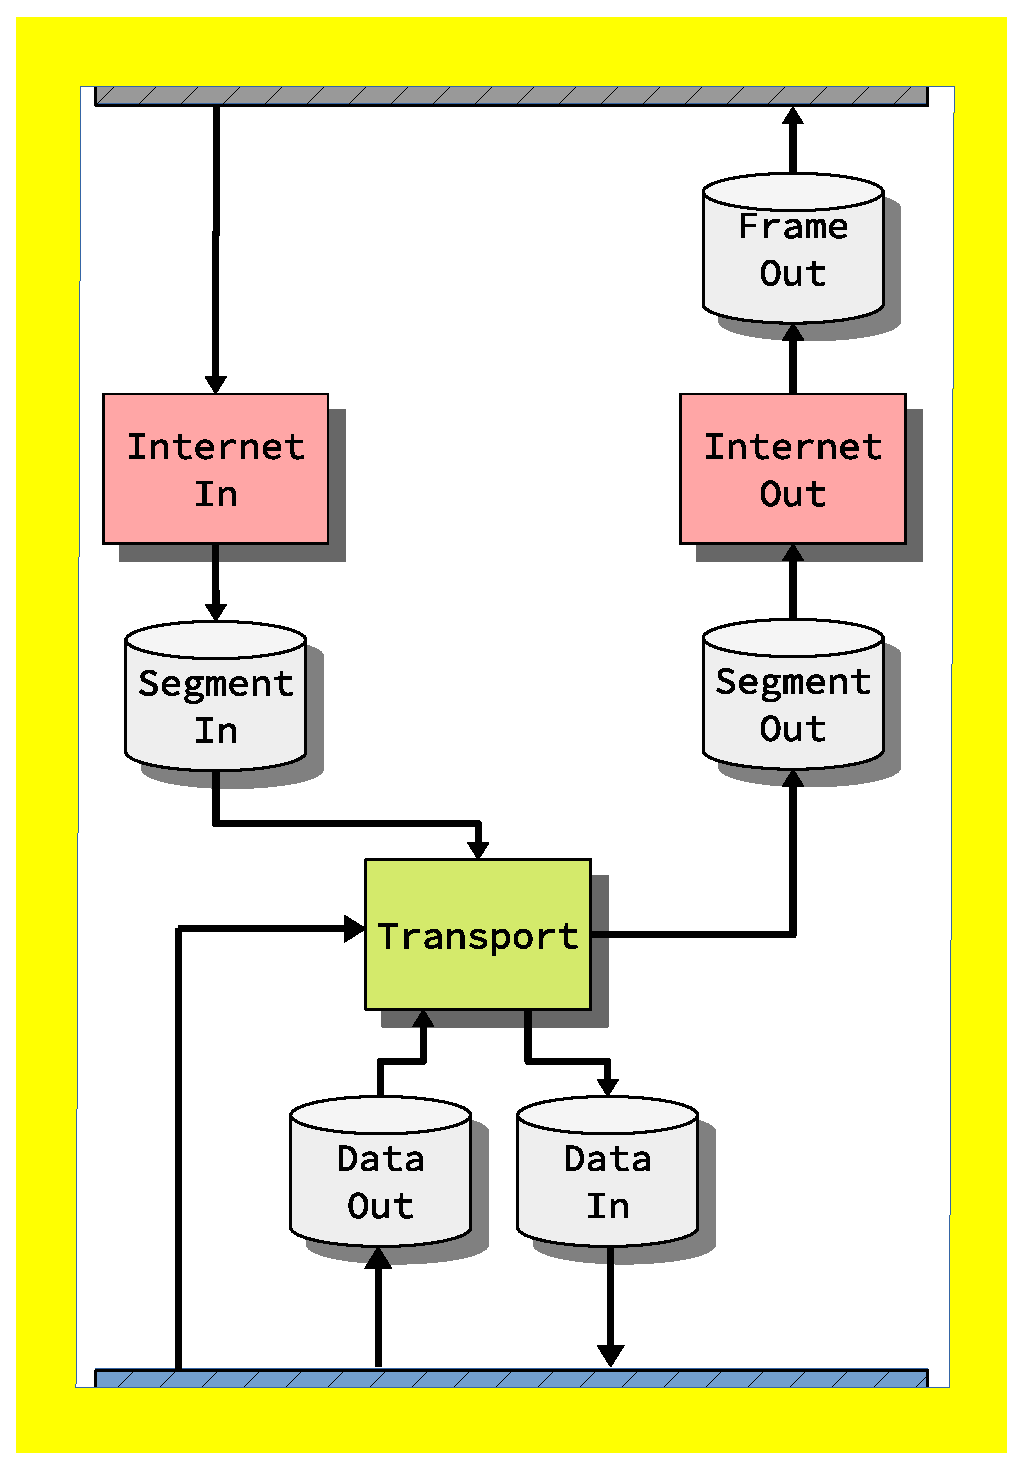
\includegraphics[width=\textwidth]{implementation/design_2_sme.eps}}
    \end{textblock*}
    \frametitle{\ImplementationTitle}
    \subsection{SME introduction}
    \framesubtitle{SME introduction}

    \begin{block}{SME(Synchronous Message Exchange) introduction}
        \begin{itemize}
            \item Processes and Busses
            \item Higher abstraction
            \item Handling of clocks
            \item Easy testing
            \item Not fully feature complete with C\#(No threads, no allocation)
        \end{itemize}
    \end{block}

\end{frame}
\note{
    \begin{itemize}
        \item What is a bus and a process
        \item No VHDL code
        \item Clocks abstracted away behind the management of processes and busses
        \item Testing straight in the simulator, but also in afterwards in the GHDL
              compiler, via an clock lookup table
        \item Since not feature complete, only simple structures can be used. We choose
              state diagrams since they are possible to make, and easy to understand
    \end{itemize}
}
\begin{frame}[fragile]
    \begin{textblock*}{\displayThumbnail}(\paperwidth-\displayThumbnail-0.2cm,0cm) % {block width} (coords)
        \colorbox{white}{\includegraphics[width=\textwidth]{implementation/design_2_state.eps}}
    \end{textblock*}
    \frametitle{\ImplementationTitle}
    \subsection{Processes}
    \framesubtitle{Processes}
    State machines\\\\
    %\begin{onlyenv}<2>
    \begin{minipage}[t]{0.3\textwidth}
        \begin{mintedcsharp}
            public class SomeProcess : StateProcess
            {
              private override async Task OnTickAsync()
              {
                a();
                await ClockAsync();
                b();
                await ClockAsync();
                c();
                await ClockAsync();
              }
            }
        \end{mintedcsharp}
    \end{minipage}%
    %\end{onlyenv}%
    \hfill%
    \begin{minipage}[t]{0.3\textwidth}
        \begin{mintedcsharp}
            public class SomeProcess : SimpleProcess
            {
            // Initial state
            state = A;

            protected override void OnTick()
            {
              switch(state) {
                case A:
                  a();
                  state = B;
                case B:
                  b();
                  state = C;
                case C:
                  c();
                  state = A;
              }
            }
        \end{mintedcsharp}
    \end{minipage}%
    \hfill%
    \begin{minipage}[t]{0.3\textwidth}
        \begin{figure}
                \centering
                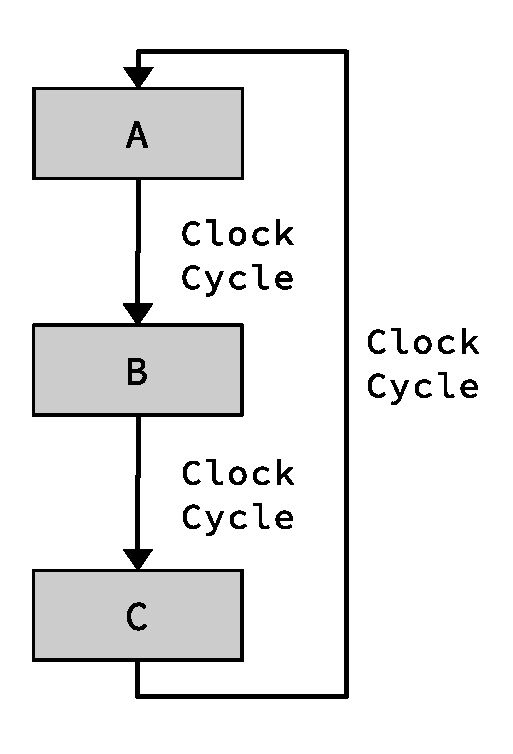
\includegraphics[scale=0.45]{implementation/empty_process_fsm.eps}
        \end{figure}
    \end{minipage}
    %\Put(-50,0){\colorbox{white}{\includegraphics[width=0.2\textwidth]{implementation/design_2_state.eps}}}

\end{frame}

\note{
State machines\\
\begin{itemize}
    \item \texttt{StateProcess}\\
          Eksekvering kan stoppes når som helst(i bidder)
    \item \texttt{SimpleProcess}\\
          Run er en clock altid, state machine håndteres
          med en switchcase. Algoritme kan splittes op i flere bidder,
          men kræver en state per bid

\end{itemize}
}

\begin{frame}[fragile]
    \begin{textblock*}{\displayThumbnail}(\paperwidth-\displayThumbnail-0.2cm,0cm) % {block width} (coords)
        \colorbox{white}{\includegraphics[width=\textwidth]{implementation/design_2_state_specific.eps}}
    \end{textblock*}
    \frametitle{\ImplementationTitle}
    \framesubtitle{Processes}
    Examples\\
    \begin{minipage}[t]{0.5\textwidth}
        \begin{figure}
            \centering
            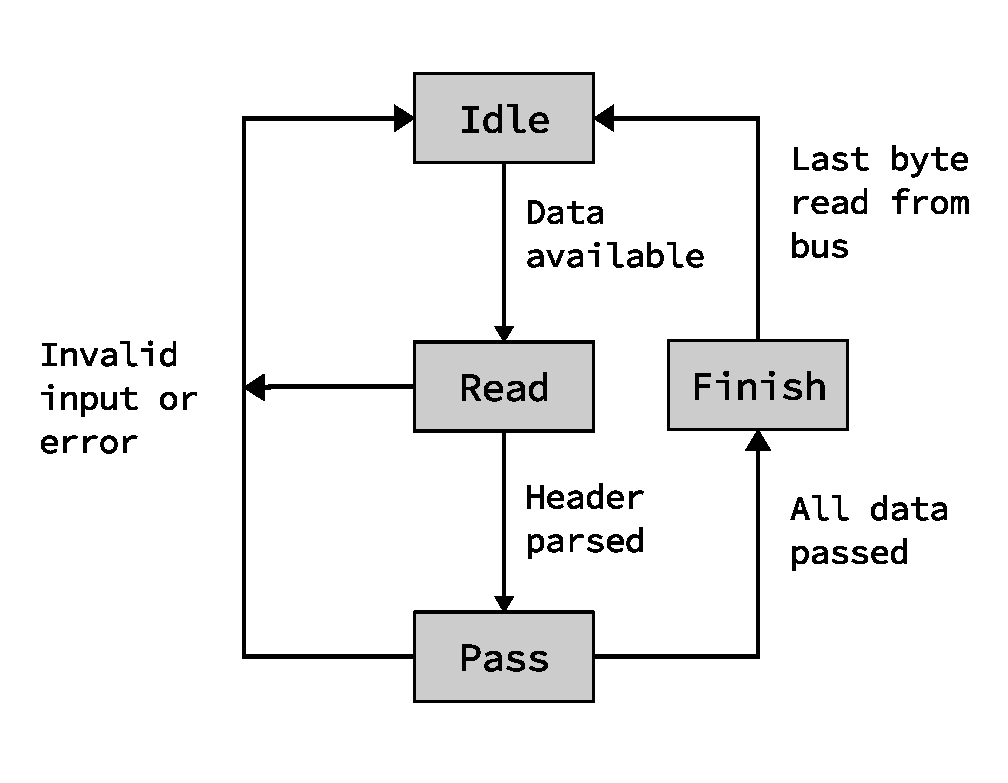
\includegraphics[scale=0.35]{implementation/internet_in_fsm.eps}
            Internet in process state machine
        \end{figure}
    \end{minipage}%
    \hfill%
    \begin{minipage}[t]{0.5\textwidth}
        \begin{figure}
            \centering
            \includegraphics[scale=0.35]{implementation/transport_fsm.eps}
            Transport process state machine
        \end{figure}
    \end{minipage}
\end{frame}
\note{

    \begin{itemize}
        \item Gå igennem state diagrammer
        \item Snak om grundlaget for de forskellige typer brug
    \end{itemize}
}

\begin{frame}[fragile]
    \begin{textblock*}{\displayThumbnail}(\paperwidth-\displayThumbnail-0.2cm,0cm) % {block width} (coords)
        \colorbox{white}{\includegraphics[width=\textwidth]{implementation/design_2_memory.eps}}
    \end{textblock*}
    \frametitle{\ImplementationTitle}
    \subsection{Buffers}
    \framesubtitle{Buffers}
    \begin{block}{Why buffers?}
        \begin{itemize}
            \item Fixes segmentation
            \item Processes can get data at their leisure
        \end{itemize}
    \end{block}

\end{frame}
\note{Hvorfor bruer vi buffers?}


\begin{frame}[fragile]
    \begin{textblock*}{\displayThumbnail}(\paperwidth-\displayThumbnail-0.2cm,0cm) % {block width} (coords)
        \colorbox{white}{\includegraphics[width=\textwidth]{implementation/design_2_memory.eps}}
    \end{textblock*}
    \frametitle{\ImplementationTitle}
    \framesubtitle{Buffers}
    Memory segments\\
    \begin{minipage}[t]{1\textwidth}
        \begin{figure}
                \centering
                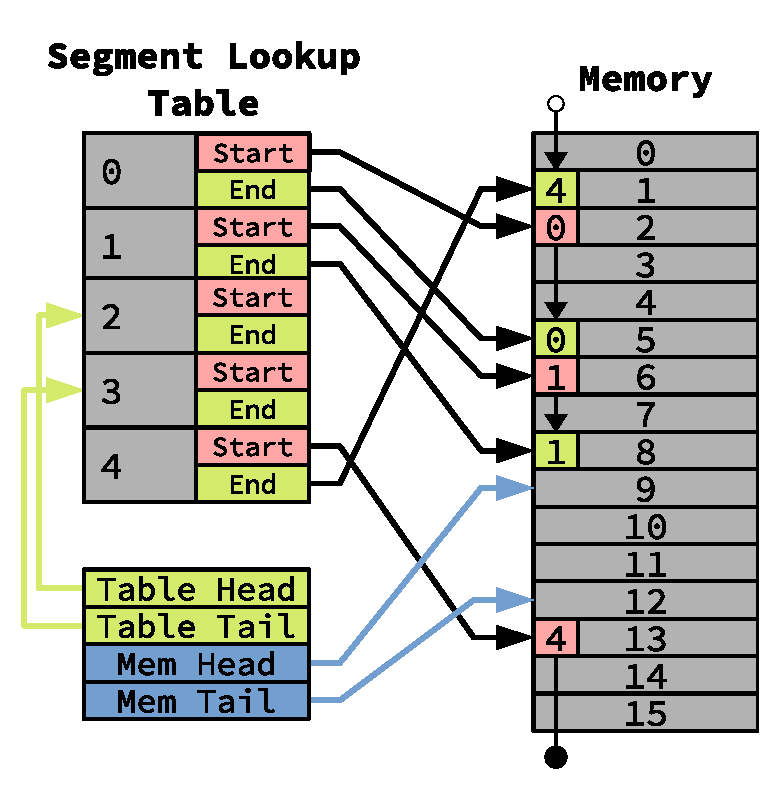
\includegraphics[scale=0.50]{implementation/memory_segments.eps}
        \end{figure}
    \end{minipage}
\end{frame}
\note{
    \begin{itemize}
        \item Reason behind?
        \begin{itemize}
            \item Segment handling
            \item References to other segment to concatting of segments later
        \end{itemize}
    \end{itemize}

}

\begin{frame}[t]
    \note<1->{Snak om input
}
    \begin{textblock*}{\displayThumbnail}(\paperwidth-\displayThumbnail-0.2cm,0cm) % {block width} (coords)
        \colorbox{white}{\includegraphics[width=\textwidth]{implementation/design_2_memory_dictionary.eps}}
    \end{textblock*}
    \frametitle{\ImplementationTitle}
    \framesubtitle{Buffers}
    Memory dictionary
    \begin{columns}[t]
        \begin{column}{0.5\linewidth}
            \begin{figure}
                \centering
                \begin{overlayarea}{\textwidth}{\textheight}
                    \only<1>{\includegraphics[width=\textwidth]{./implementation/memory_dictionary/memory_dictionary_multi_0.eps}}
                    \only<2>{\includegraphics[width=\textwidth]{./implementation/memory_dictionary/memory_dictionary_multi_1.eps}}%
                    \only<3>{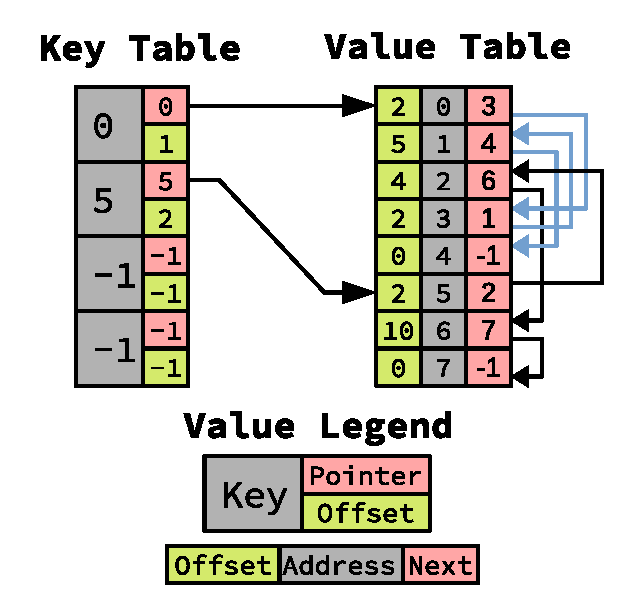
\includegraphics[width=\textwidth]{./implementation/memory_dictionary/memory_dictionary_multi_2.eps}}%
                \end{overlayarea}
            \end{figure}
        \end{column}

        \begin{column}{0.3\linewidth}
            \\
            \only<1>{
                Initial state.\\
                Key \texttt{5} have 2 elements:\\
                $$[4,18]$$
                at index:
                $$[2,7]$$
            }
            \only<2>{
                Insert element 8:
                Key \texttt{5} have 3 elements:\\
                $$[4,8,18]$$
                at index:
                $$[2,6,7]$$
            }
            \only<3>{
                Insert element 2:
                Key \texttt{5} have 4 elements:\\
                $$[2,4,8,18]$$
                at index:
                $$[5,2,6,7]$$
            }
        \end{column}
        \begin{column}{0.2\linewidth}
        \end{column}
    \end{columns}
\end{frame}



\begin{frame}[fragile]
    \note<1->{Overflow!\\
    kan læses ved:
    \begin{itemize}
        \item Kør løkken en gang per clock
        \item Brug en anden model end en linked list, måske et fast offset?
    \end{itemize}
    }
    \begin{textblock*}{\displayThumbnail}(\paperwidth-\displayThumbnail-0.2cm,0cm) % {block width} (coords)
        \colorbox{white}{\includegraphics[width=\textwidth]{implementation/design_2_memory.eps}}
    \end{textblock*}
    \frametitle{\ImplementationTitle}
    \framesubtitle{Buffers}
    Some problems with the memory dictionaries!
    \begin{figure}
        \centering
        \begin{overlayarea}{0.76\textwidth}{\textheight}
            \only<1>{\includegraphics[width=\textwidth]{./implementation/memory_overrun/memory_overrun_0.eps}}
            \only<2>{\includegraphics[width=\textwidth]{./implementation/memory_overrun/memory_overrun_1.eps}}%
            \only<3>{\includegraphics[width=\textwidth]{./implementation/memory_overrun/memory_overrun_2.eps}}%
            \only<4>{\includegraphics[width=\textwidth]{./implementation/memory_overrun/memory_overrun_3.eps}}%
            \only<5>{\includegraphics[width=\textwidth]{./implementation/memory_overrun/memory_overrun_4.eps}}%
            \only<6>{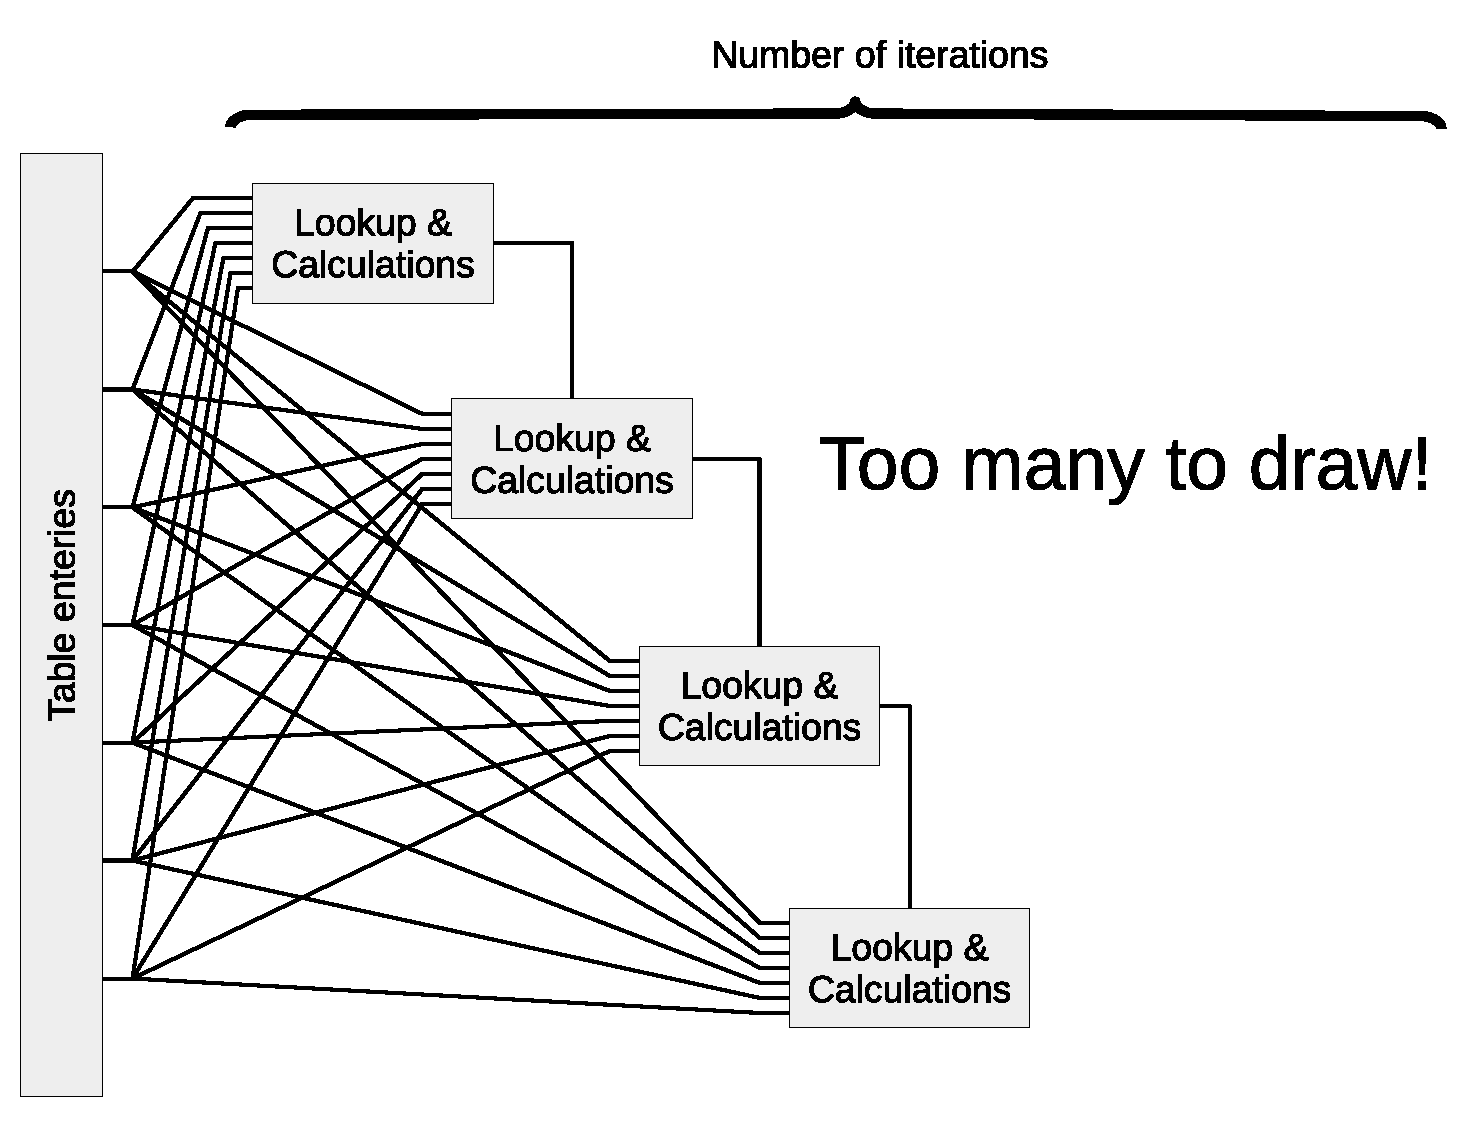
\includegraphics[width=\textwidth]{./implementation/memory_overrun/memory_overrun_5.eps}}%
        \end{overlayarea}
    \end{figure}
\end{frame}


\begin{frame}[fragile]
    \begin{textblock*}{\displayThumbnail}(\paperwidth-\displayThumbnail-0.2cm,0cm) % {block width} (coords)
        \colorbox{white}{\includegraphics[width=\textwidth]{implementation/design_2_busses.eps}}
    \end{textblock*}
    \frametitle{\ImplementationTitle}
    \subsection{Interface signal protocol}
    \framesubtitle{Interface signal protocol}
Identifying the scenarios

\centering
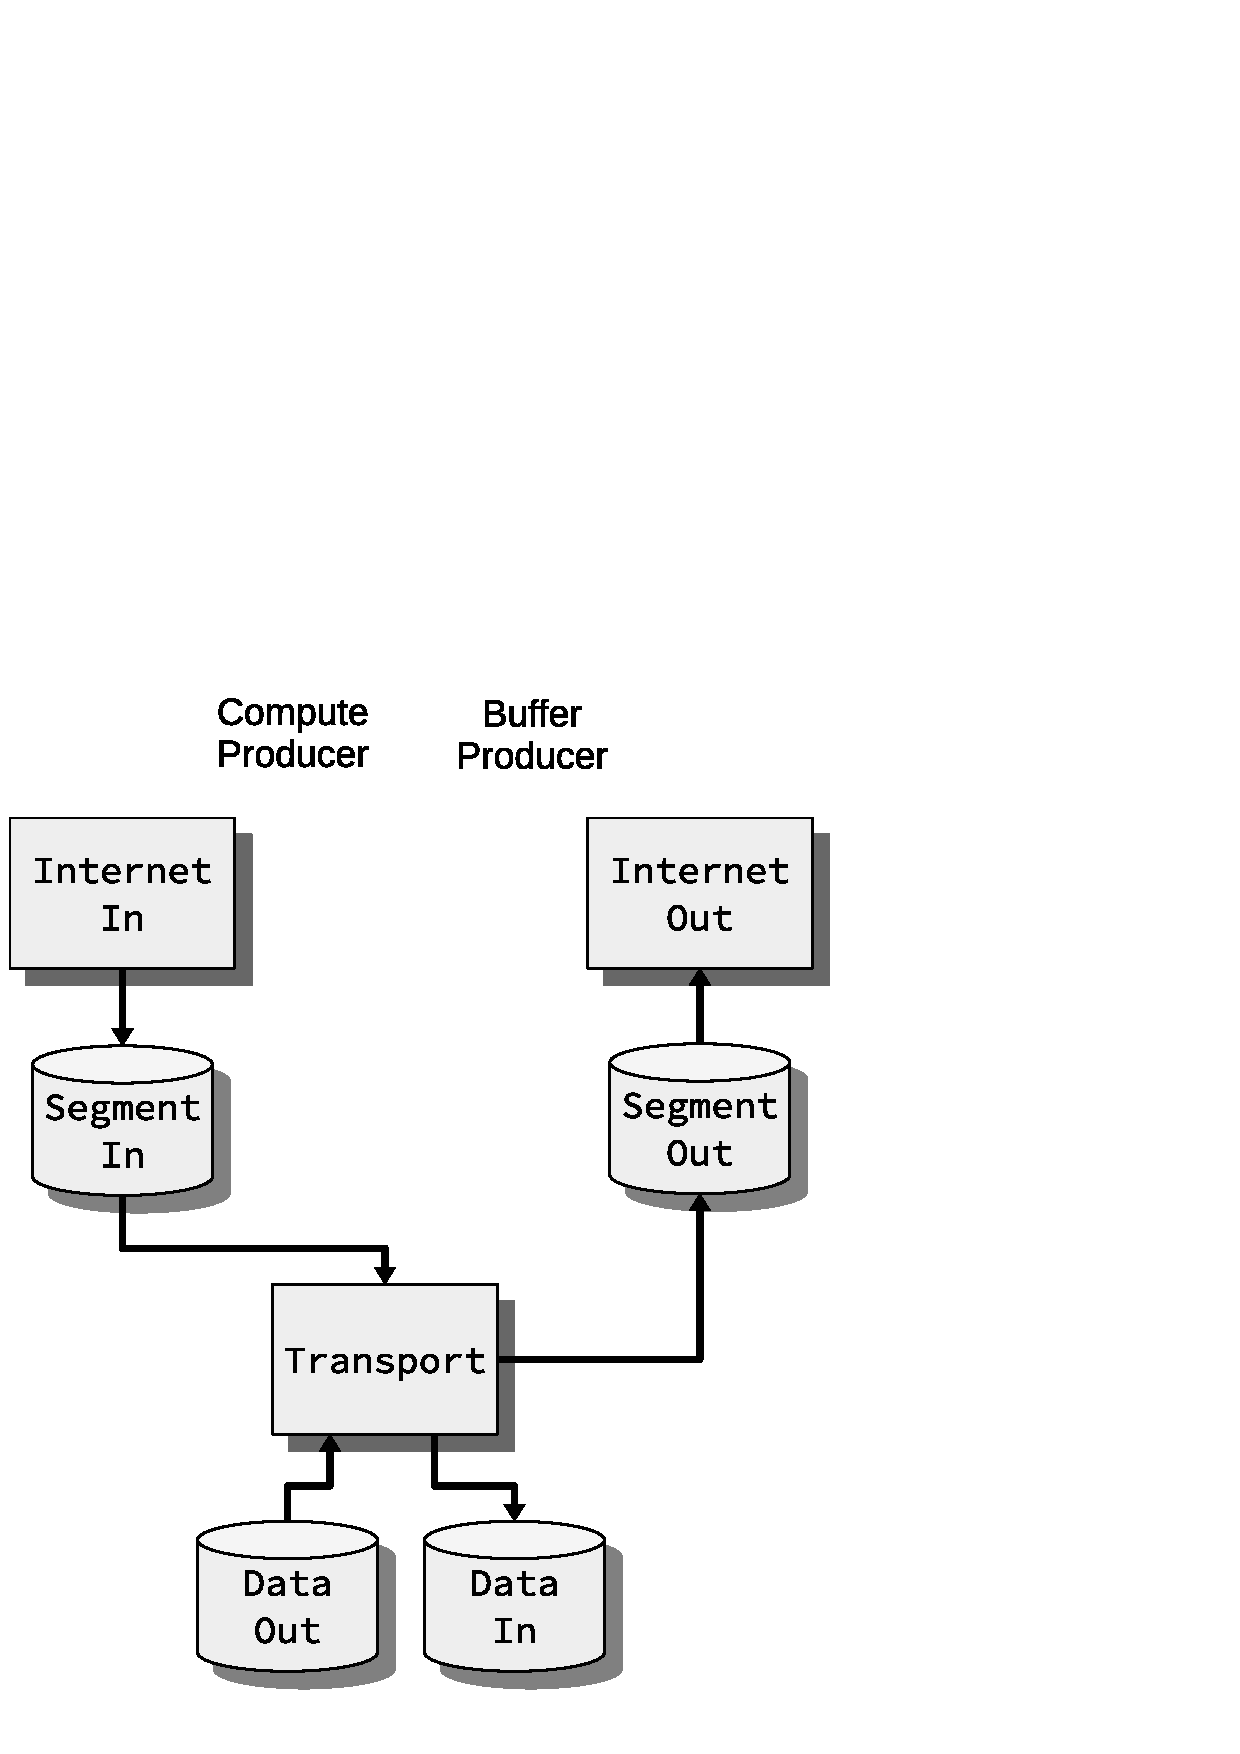
\includegraphics[scale=0.40]{implementation/signal_protocol_identification.pdf}

\end{frame}

\note{Data skal overføres hurtigst muligt, og det må ikke gå tabt\\

2 scenarier: fra "compute" til buffer, og omvendt \\

- CP kan ikke vente\\
- BP har stor buffer, og consumer starter transaktion


}


\begin{frame}[fragile]
    \begin{textblock*}{\displayThumbnail}(\paperwidth-\displayThumbnail-0.2cm,0cm) % {block width} (coords)
        \colorbox{white}{\includegraphics[width=\textwidth]{implementation/design_2_busses.eps}}
    \end{textblock*}
\frametitle{\ImplementationTitle}
\framesubtitle{Interface signal protocol}
\begin{figure}
        \centering
        \includegraphics[scale=0.35]{implementation/compute_producer.eps}
\end{figure}

\end{frame}




\begin{frame}[fragile]
    \begin{textblock*}{\displayThumbnail}(\paperwidth-\displayThumbnail-0.2cm,0cm) % {block width} (coords)
        \colorbox{white}{\includegraphics[width=\textwidth]{implementation/design_2_busses.eps}}
    \end{textblock*}
    \frametitle{\ImplementationTitle}
    \framesubtitle{Interface signal protocol}
    \textbf{Buffer-Producer:} Inspired by AXI4\\
    \begin{figure}
                \includegraphics[scale=0.7]{implementation/axi4_handshake.eps}

        \end{figure}
\end{frame}


\begin{frame}[fragile]
    \begin{textblock*}{\displayThumbnail}(\paperwidth-\displayThumbnail-0.2cm,0cm) % {block width} (coords)
        \colorbox{white}{\includegraphics[width=\textwidth]{implementation/design_2_busses.eps}}
    \end{textblock*}
    \frametitle{\ImplementationTitle}
    \framesubtitle{Interface signal protocol}
        \begin{figure}
                \centering
                \includegraphics[scale=0.35]{implementation/buffer_producer.eps}
       \end{figure}
\end{frame}




% \begin{frame}[fragile]
%     \frametitle{\ImplementationTitle}
%     \framesubtitle{Interface protocol}
%     The interface structures\\
%     \begin{minipage}[t]{0.4\textwidth}
%         \begin{mintedcsharp}
%             enum InterfaceFunction : byte
%             {
%                 INVALID = 0,
%                 // BIND = 1,
%                 LISTEN = 2,
%                 CONNECT = 3,
%                 ACCEPT = 4,
%                 CLOSE = 7,
%                 // ...
%                 OPEN = 255,
%             }
%
%             struct InterfaceData
%             {
%                 public int socket;
%                 public uint ip;
%                 public byte protocol;
%                 public ushort port;
%             }
%         \end{mintedcsharp}
%     \end{minipage}%
%     \hfill%
%     \begin{minipage}[t]{0.4\textwidth}
%         \begin{mintedcsharp}
%             interface InterfaceBus : IBus
%             {
%                 bool valid;
%                 byte interface_function;
%                 InterfaceData request;
%             }
%
%             interface InterfaceControlBus : IBus
%             {
%                 bool valid;
%
%                 byte exit_status;
%                 byte interface_function;
%                 InterfaceData request;
%                 InterfaceData response;
%             }
%         \end{mintedcsharp}
%     \end{minipage}
% \end{frame}
%
%
% \begin{frame}%[fragile]
%     \frametitle{\ImplementationTitle}
%     \framesubtitle{Interface protocol}
%     Limitations
%     \begin{itemize}
%         \item One request at a time.
%         \item Arbitrary delay between request and response.
%     \end{itemize}
% \end{frame}

\chapter{Evaluation}
\label{chap:evaluation}
%\noteinfo[inline]{Remember to describe that we could not get the network stack down on the FPGA}
\section{Setup}
In the initial stages of testing, the components had simulation processes between
each modules. This made it possible to implement different modules of the system
independent of each other.\\

These tests were changing a lot because the initial design was not
reached.
When the modules were done, they were wired together and a simulator
was created to handle all input and output of the network stack.

\subsection{Graph file simulator}
\begin{figure*}%[!ht]
    \centering
    \begin{subfigure}[b]{0.16\textwidth}
        \centering
        \includegraphics[scale=0.45]{evaluation/dot_files/datain.eps}
        \caption{Data In}
        \label{fig:packet_graph_datain}
    \end{subfigure}%
    \begin{subfigure}[b]{0.16\textwidth}
        \centering
        \includegraphics[scale=0.45]{evaluation/dot_files/send.eps}
        \caption{Send}
        \label{fig:packet_graph_send}
    \end{subfigure}%
    \begin{subfigure}[b]{0.16\textwidth}
        \centering
        \includegraphics[scale=0.45]{evaluation/dot_files/command.eps}
        \caption{Command \protect\footnotemark}
        \label{fig:packet_graph_command}
    \end{subfigure}%
    \begin{subfigure}[b]{0.16\textwidth}
        \centering
        \includegraphics[scale=0.45]{evaluation/dot_files/dataout.eps}
        \caption{Data Out}
        \label{fig:packet_graph_dataout}
    \end{subfigure}%
    \begin{subfigure}[b]{0.16\textwidth}
        \centering
        \includegraphics[scale=0.45]{evaluation/dot_files/receive.eps}
        \caption{Receive}
        \label{fig:packet_graph_receive}
    \end{subfigure}%
    \begin{subfigure}[b]{0.16\textwidth}
        \centering
        \includegraphics[scale=0.45]{evaluation/dot_files/wait.eps}
        \caption{Wait}
        \label{fig:packet_graph_wait}
    \end{subfigure}%
    \caption{The different node types in the simulation graph}
    \label{fig:packet_dot_files}
\end{figure*}%
The graph file simulator is an abstract structure for easily composition and
illustrations of simulations in the system. The system can be boiled down
to inputs(sources) and output(sinks). The code is deterministic, since the same
combination of input and output signals would result in the exact same internal
state of the system. This means that a simulation of the system as a whole would
require knowing what to write/read at every source/sink, and doing it at the
right time. However, we do not need the timing on a clock to clock basis, since
the external network does not care when the system sends out a packet, only
if the packet is structured correctly. The user however may need information
regarding the latency of the system. The latency is based on the
specific system state, and is described in
\autoref{subsec:latency}.\\
With these assumptions it is possible to illustrate the timeline of the packets
with a graph, where a vertex does action on a clock to clock basis(etc. sending a
packet into the system.), and each edge describes what node to proceed to.
Each vertex have a state. When the \texttt{Done} state is reached
the next vertex is set to the \texttt{Ready} state, but only if
they are connected via an edge. If a vertex contains multiple ingoing edges, each
vertex with outgoing edges to that vertex needs to be \texttt{Done}.\\
{\renewcommand{\arraystretch}{1.3}
\begin{table}[htpb]
    \begin{center}
        \begin{tabular}{lcc}
            State & Color&Description\\ \hline \hline
            \texttt{Waiting}& \statecolorbox{graph_waiting} &
            \makecell{Vertex is not in use.}\\ \hline

            \texttt{Ready}& \statecolorbox{graph_isready} &
            \makecell{Vertex Is ready\\ for activation.}\\ \hline

            \texttt{Active}& \statecolorbox{graph_active} &
            \makecell{Vertex is active.\\ Simulator is\\ gathering data.}\\ \hline

            \texttt{Inactive}& \statecolorbox{graph_inactive} &
            \makecell{Vertex is inactive.\\Simulator is not\\ gathering data.}\\ \hline

            \texttt{Done}& \statecolorbox{graph_done} &
            \makecell{Vertex is done\\ and validated.}
        \end{tabular}
    \end{center}
    \caption{The different states of the nodes, and their respective colors
    used for illustration.} \label{tab:graph_node_states}
  \end{table}
}\\
Each vertex have their own type, defining what input source or output sink to
use. The graph file simulator consists of multiple input sources and output sinks
as seen in \autoref{fig:packet_dot_files}.\\
There are three inputs giving data to the system:
Data in(\subref{fig:packet_graph_datain}),
Send(\subref{fig:packet_graph_send}) and
Command(\subref{fig:packet_graph_command}).
There are two sinks getting data from the system
Data out(\subref{fig:packet_graph_dataout}) and
Receive(\subref{fig:packet_graph_receive}).
The node type Wait(\subref{fig:packet_graph_wait}) is special, since
it does not use an input or a sink. It simply counts down each clock, until its
counter reaches zero.\\
Since there only exist one of each input source and output sink (except Wait),
the simulator can only work on one vertex of each type at a time.
In graphs that consists of multiple ready vertexes of same type, the vertex with
the lowest ID are focused on first. When a vertex is focused, it is set as
\texttt{Active}.\\
When the vertex is finished, it is set to \texttt{Done}.
An example of a graph can be seen in
\autoref{fig:graph_simulation_running_examples}.


\begin{figure*}[htpb]
    \centering
    \begin{subfigure}[b]{0.5\textwidth}
        \centering
        \includegraphics[scale=0.45]{evaluation/dot_files/example_graph_initial.eps}
        \caption{The initial state of a simulation}
        \label{fig:example_packet_graph_initial}
    \end{subfigure}%
    \begin{subfigure}[b]{0.50\textwidth}
        \centering
        \includegraphics[scale=0.45]{evaluation/dot_files/example_graph_running.eps}
        \caption{The state after 1005 clocks}
        \label{fig:example_packet_graph_running}
 	\end{subfigure}%
    \caption{A Illustration of the graph states before running and 1005 clocks
    inside the simulation}
    \label{fig:graph_simulation_running_examples}
\end{figure*}

\subsection{VHDL code}
%\notejan{should we add more to this?}
One of the biggest advantages of \gls{sme} is its easy testing, and its
compilation to VHDL code. By using the GHDL project
\cite{github_ghdl}.
By using the GHDL project, the generated VHDL code can be simulated to ensure
that it is clock cycle accurate with the SME simulation. SME generates a table
of signals on a clock by clock basis, that is tested up against the GHDL code.
%\notemark{"By using the GHDL project, the generated VHDL code can be simulated to ensure that it is clock cycle accurate with the SME simulation" - eller noget i den dur}
Unfortunately, our code does not compile into \gls{vhdl}.


\section{Test}
\footnotetext{This block is not implemented in the codebase}
% OBS, footnote text here from fig:packet_dot_files. needs to be on same page to work
To test the system we recorded a setup of packets containing both \gls{udp} and
\gls{tcp} packets, with focus on the \gls{udp} packets. There are three
\gls{udp} connections, and three \gls{tcp} connections. Two of the \gls{udp}
connections contain valid ports (6543,6789) and one contains an invalid port (3456).\\
Each of the valid \gls{udp} connections where hardcoded into the test, so there where no
need for command blocks(\autoref{fig:packet_graph_command}).
In the illustration at \autoref{fig:graph_simulation_running_examples} the
same test is run, but with only $4*2$ good \gls{udp} packets, $4$ bad, and
no \gls{tcp} packets\\
When data is received from \texttt{Data In}, the same data is copied and
sent to \texttt{Data Out}. \\
In the example 6 packets have been sent into the system, and number 7(Id 70)
is \texttt{Active}. The active \texttt{Send} block is giving its 30'th byte
with a hex value of 0x21.\\
The real test had 17283 packets in total, where 1920 of those where udp packets.
Of the udp packets $2/3$ (1280) where the valid ports. The data sent
through \texttt{Internet In} totals 1832958 Bytes.\\
The test took around 1.83 million clocks to finish. This indicates that the system
did handle all incoming packets in real time without having to break the input,
even when sending limited amounts of data out.



\section{Verification}
\subsection{Latency}\label{subsec:latency}
There are several factors when calculating the latency of the system.
\begin{description}
    \item[$n_{\mathtt{D}}$]:\quad
    The number of bytes in the data part of the protocol. This excludes both
    headers from transport and internet.
    \item[$n_{\mathtt{I}}$]:\quad
    The internet header size.
    \item[$n_{\mathtt{T}}$]:\quad
    The transport header size.
    \item[$n$]:\quad
    The total packet size.
\end{description}
When a packet is propagating through the system, most
of the latency comes from the buffers. All processes that connects
to a buffer, does work, and submits to a buffer.
When possible, processes will pass the data straight ahead. For example, the
\texttt{Transport} process will first pass the data from \texttt{Data Out} to
the \texttt{Segment Out}, and then send the header. The passing state happens
while reading from the buffer. This only adds two clock cycles of delay between
\texttt{Data Out} and \texttt{Segment out}.
In the following cases, we assume a simple system where either only packets are
being sent, or packets are being received.

\subsubsection{From Recive to Data In}
When the system starts to receive the first byte of a packet, to the last byte read from
the user. This case uses \gls{ipv4} internet header, and \gls{udp} transport
header.
% This formular can also be used in other transport headers, such as \gls{tcp}.
% To make it work with \gls{tcp}, one would need to calculate the constant $C$,
% based on \gls{tcp} specific features such as how long are the sequence of
% SYN/ACK \notemark{Carl var ogsaa forvirret over denne del. Jeg synes vi skal
% slette TCP fra beregningen, for den er slet ikke implementeret.} takes.
\begin{equation*}
    2 + n + 2 + (n_{\mathtt{D}} + n_{\mathtt{T}}) + 2 + n_{\mathtt{D}}
\end{equation*}
That simplifies down to
\begin{equation} \label{eq:receive_to_datain}
     6 + n_{\mathtt{I}} + 2n_{\mathtt{T}} + 3n_{\mathtt{D}}
\end{equation}
\subsubsection{From Data out to Send}
Making the system send out data makes the formular a bit different. The outgoing
packets goes through an extra buffer.
\begin{equation*}
   2 + n_{\mathtt{D}} + 2 + (n_{\mathtt{D}} + n_{\mathtt{T}}) + 2 + n + 2 + n
\end{equation*}
That simplifies down to
\begin{equation} \label{eq:dataout_to_send}
    8 + 2n_{\mathtt{I}} + 3n_{\mathtt{T}} + 4n_{\mathtt{D}}
\end{equation}

\subsubsection{Observations}
%\notemark{Noget andet, som i ikke har nævnt, at det i skriver er latency fra data kommer ind/ud til den er færdig. Jeres løsning er vel pipelinet, så efter start latency, så kan i vel blive ved med at feede netværket (hvad enten det er ind eller ud) ? }
It is clear when comparing \autoref{eq:dataout_to_send} and
\autoref{eq:receive_to_datain} that sending packets have a higher latency than
receiving packets. This is clearly because of the added buffer.\\
It is also important to note that the first packet through the system gets the
full latency. However the next packet will not have to wait for the first packet
to propagate through the system. Since the system is pipelined, the packet
can be gathered by the buffers right after the last packet.\\
It is not clear
from the latency formulars that receiving data "cuts" off data from the packet
at each buffer step. This makes it possible to receive data at a constant pace,
without filling the buffers. On the other hand sending out packets are
problematic. \\
Since each step adds additional information to the packet, the \texttt{Data Out}
buffer may fill faster than it can be emptied.


\subsection{Outgoing packet validation}

\begin{figure}[h]
\centering
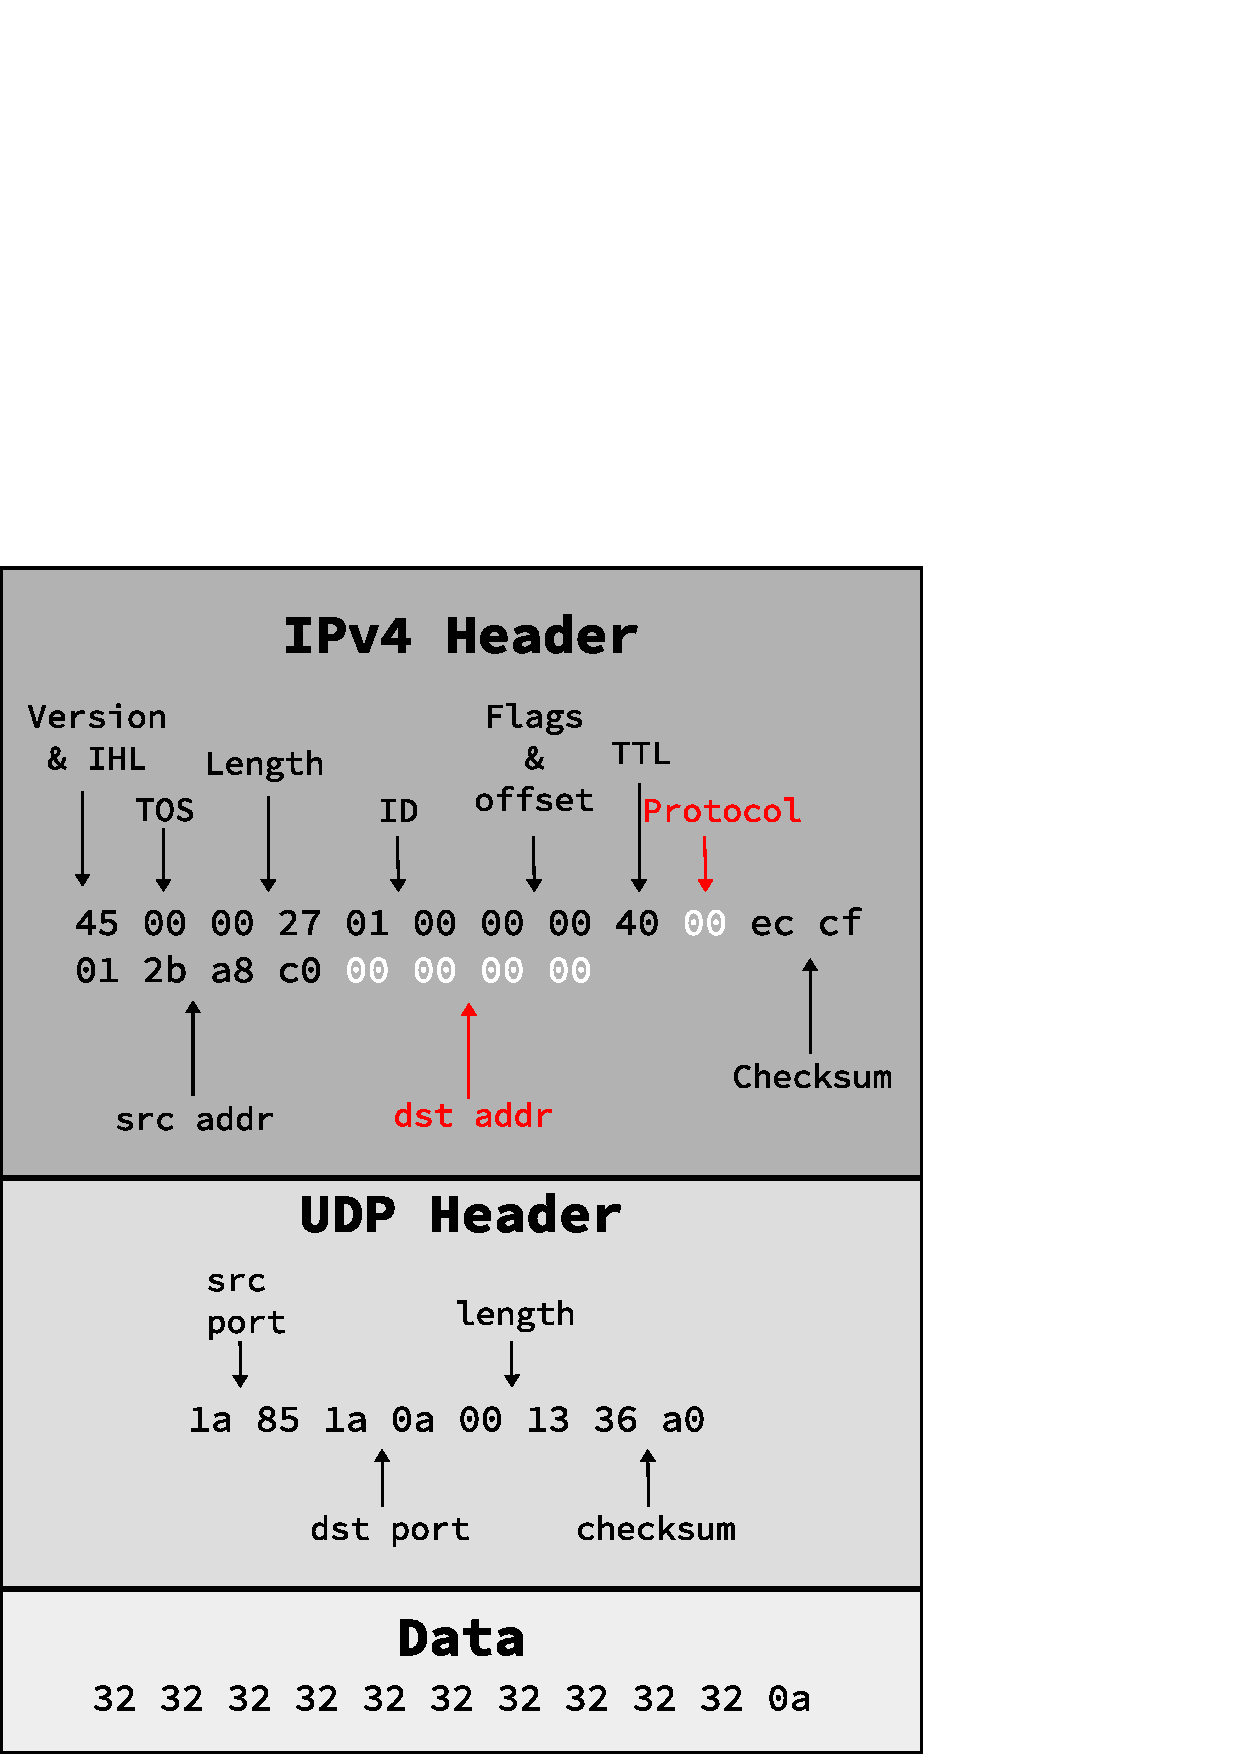
\includegraphics[width=\linewidth]{evaluation/hexdump.pdf}
	\caption{The hexadecimal representation of one of the outgoing packets
	generated by the system. Notice the red fields, indicating an error.}
\label{fig:packet_hexdump}
\end{figure}

The test has demonstrated that the packets themselves arrive at their
appropriate destinations intact. The test-suite tests all the supported
features, such as various protocols, port numbers, multiple connections through
sockets, etc.

To verify that the outgoing packets are formatted correctly, the output has
been captured and dumped into raw binary files. These can be interpreted by
numerous network utilities, such as the most well-known Wireshark.
These tools quickly detected malformations of the packets -- the
\texttt{protocol} field of the \gls{ipv4} header was not set, nor was the
destination address set. However, all offsets were calculated correctly, and
the packets had the exact proper lengths.
\autoref{fig:packet_hexdump} shows the raw binary dump of a packet, with the fields
marked.


\subsection{Internet Protocol Suite compliancy as per RFC 1122}
The networking stack was designed and implemented to comply with the networking
standards specified in RFC 1122. Although the number and size of the standards
required to be fully compliant with the Internet Protocol Suite is way over the
scope of this project, the list of requirements is a useful tool to get an
summary of the capabilities of the system.

\autoref{tab:rfc_compliance} shows a subset of the required features.
Features and protocols unrelated to this project have been removed, and can be
assumed to not be supported. The full list can be seen in \cite[Section 3.5,
Page 72]{RFC1122}.


\section{Discussion}
\begin{frame}
  \frametitle{Discussion}


\begin{columns}
\begin{column}{0.5\textwidth}
\begin{itemize}
\item<1->Performance
\item<2->Usability
\item<3->Using C\#
\end{itemize}
\end{column}

\begin{column}{0.5\textwidth}
% \includegraphics<1>[scale=0.5]{congest.eps}
\end{column}
\end{columns}





\end{frame}

\section{Conclusion}
\begin{frame}
  \frametitle{Conclusion}

\centering
Conclusion

\end{frame}

\section{Future Work}
\begin{frame}
  \frametitle{Future Work}
\framesubtitle{Firewall}
\begin{figure}
\centering
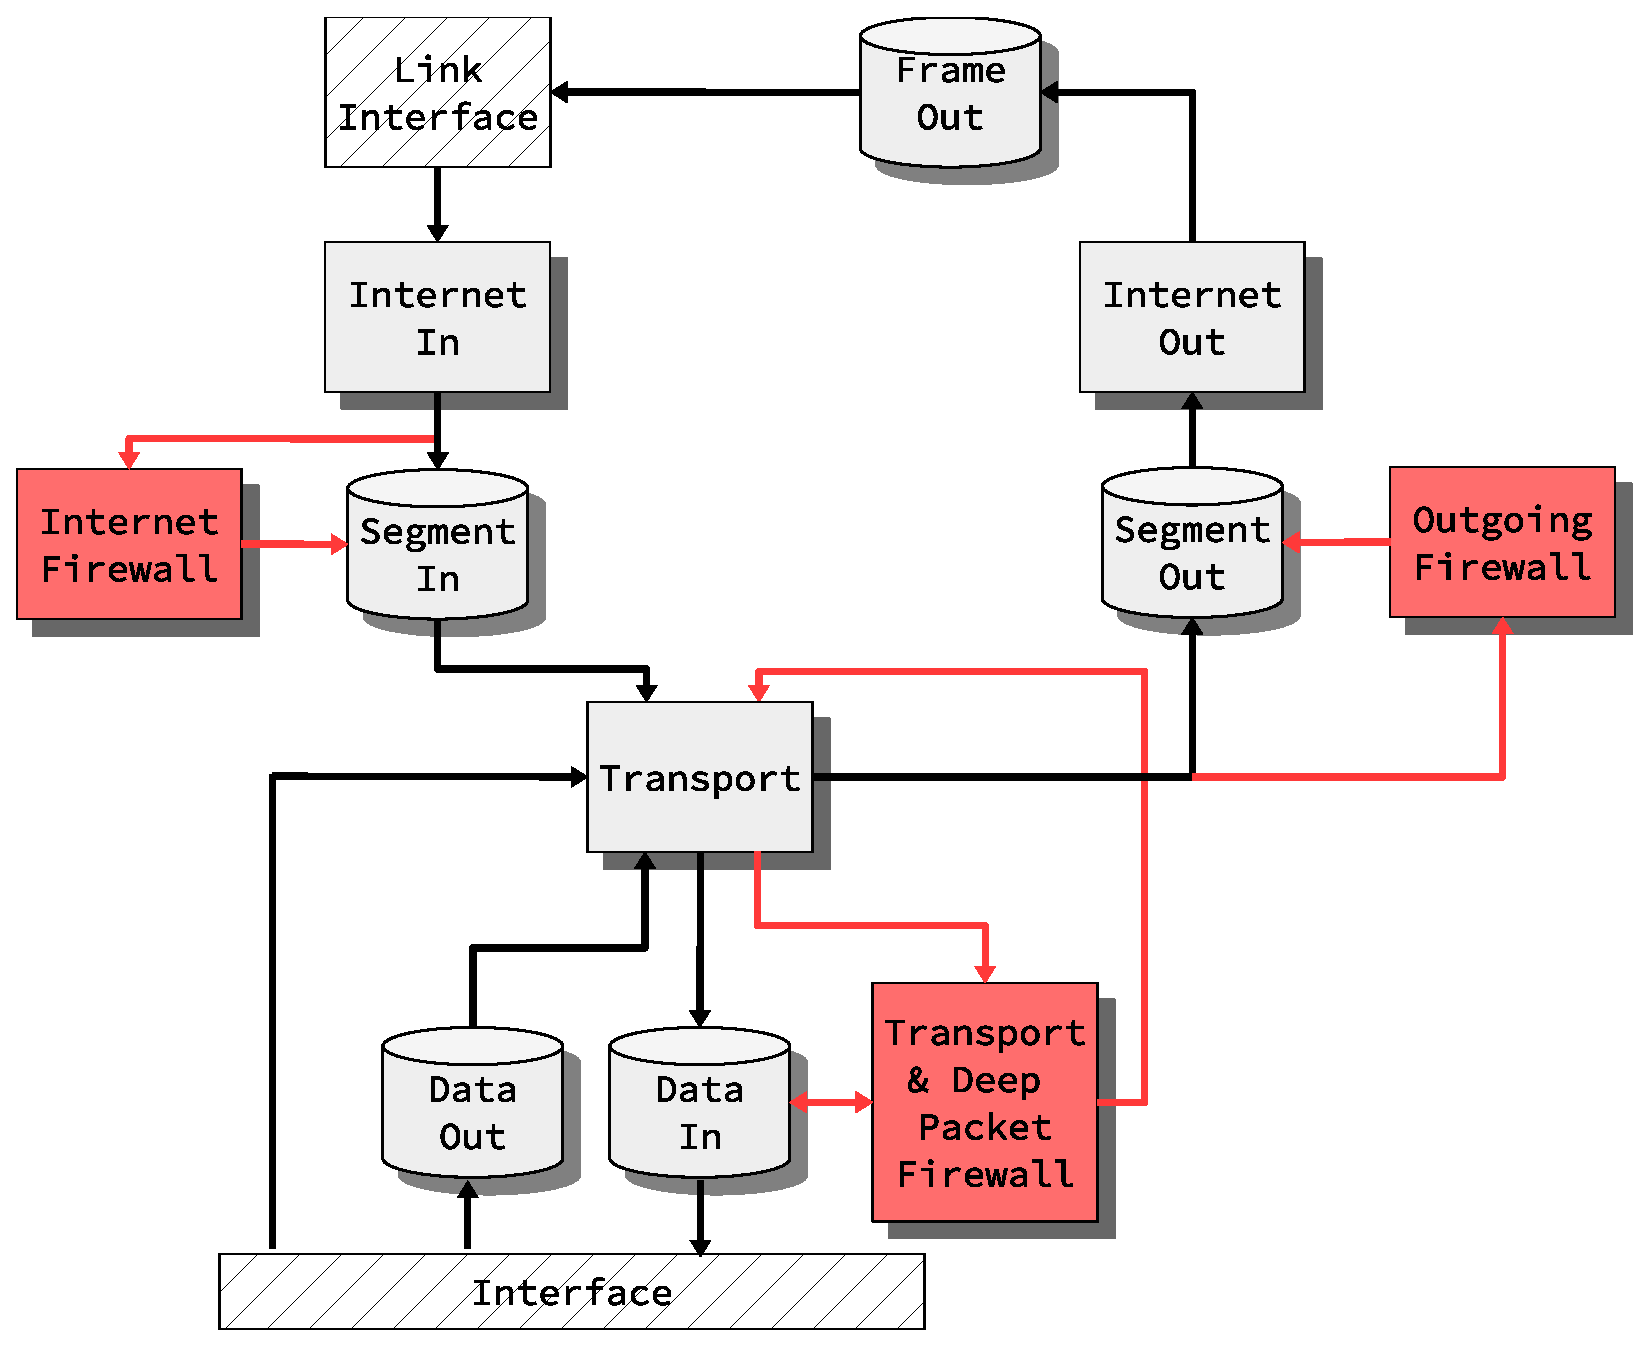
\includegraphics[scale=0.30]{../thesis/future_work/firewall_integration_design.eps}
\end{figure}
\end{frame}
\note{Integration med buffere.
Hvad ville det indebære}


\begin{frame}
  \frametitle{Future Work}
\framesubtitle{TCP}
How to implement TCP
\end{frame}












\section{Questions}
\begin{frame}{Bibliography}
\bibliographystyle{plainnat}
\setcitestyle{numbers}
\bibliography{bib}

\end{frame}


\begin{frame}
    \begin{center}
        \movie{\includegraphics[width=1\textwidth]{./demo/thumbnail.png}}{./demo/output.avi}
    \end{center}
\end{frame}



\end{document}



